\chapter{Methodology}
\label{chap:methodology}

This chapter describes how \NEMO{} was designed, implemented and verified. It
starts with the engineering research design and the functional requirements
derived from marine structural codes, shipyard fabrication practice and early
exploratory testing. It then follows a design through the tool in the order the
engine handles it. The loads and checks come first, then stock-aware sizing,
solid geometry, finite element analysis and traceable outputs. The closing
sections describe the verification suite, the desktop interface, the optional
Autodesk Fusion connector and the shipboard case studies analysed in
Chapter~\ref{chap:results}.

\section{Research design}
\label{sec:research-design}

The project followed a design-science approach. The output is a verified marine
design tool, and the three research questions in
Section~\ref{sec:research-questions} are answered by building the engineering
engine, testing its solvers against closed-form and published reference
solutions, and applying it to representative vessel design cases. The work
proceeded in four stages.

\begin{enumerate}
    \item \textbf{Marine code basis and early trials.} Design requirements were
    drawn from ASME BTH-1, AISC 360-16, IACS UR S10, ASME V\&V~10 and findings
    from early exploratory CAD and manual Fusion trials
    (Section~\ref{sec:early-testing}). These became the requirements in
    Table~\ref{tab:requirements}.
    \item \textbf{Shared engine, built part by part.} The lifting padeye was
    built end to end first so that it fixed the shared architecture, namely the
    check record, rule-set interface, stock-aware sizing pattern, CAD and
    finite element pipeline, engineering log and PDF report generator. The pipe
    support bracket and stabilizer fin then reused those shared modules.
    \item \textbf{Verification alongside development.} Each engineering
    calculation received automated tests as it was written. Hand calculations,
    closed-form beam and elasticity solutions, and published stress
    concentration and foil coefficients were assembled into a benchmark suite
    that can be rerun directly from the application.
    \item \textbf{Desktop interface and shipboard case studies.} A local
    browser interface, PDF calculation package and optional Fusion connector
    were built over the engine. Realistic vessel cases and operating-envelope
    sweeps were then executed to establish which limits govern each marine
    detail.
\end{enumerate}

\subsection{Engineering design requirements}
\label{sec:requirements}

Table~\ref{tab:requirements} sets out the nine engineering requirements that
guided the architecture of \NEMO{}, grounded in marine structural practice,
numerical verification principles \cite{asmeVV10} and the failure modes
observed during early exploratory testing.

\begin{table}[H]
\centering
\caption{Engineering and verification requirements for \NEMO{}}
\label{tab:requirements}
\small
\begin{tabularx}{\textwidth}{>{\raggedright\arraybackslash}p{0.42\textwidth}>{\raggedright\arraybackslash}X}
\toprule
\textbf{Marine engineering or verification driver} & \textbf{Requirement for \NEMO{}}\\
\midrule
Closing the design loop requires automated stress confirmation; early Fusion API trials showed that commercial simulation studies could not be set up and solved programmatically. &
R1. Three-dimensional stress analysis runs automatically inside the tool, with no manual transfer step, for every proposed design.\\
Manual transfer of loads into FEA invites unit and transcription errors (observed in an early trial where 1.472~N was entered instead of 1,472~N). &
R2. FEA loads are derived directly from the job force model, and the solver checks both force and moment equilibrium against the support reactions.\\
Design sign-off by a marine engineer or surveyor requires traceable equations rather than unsourced screening factors. &
R3. Every check states its governing equation, substituted numbers and named source, clearly separating code provisions from yard practice.\\
Stabilizer fin sizing depends on vessel speed, foil geometry and angle of attack, not an assumed static load. &
R4. Fin hydrodynamic loads are derived from operating speed, foil dimensions and angle by two independent methods, accompanied by a cavitation screen.\\
Secondary marine steelwork must comply with applicable structural lifting, piping and hull-appendage codes. &
R5. Each component is checked against a named design code (ASME BTH-1, AISC 360-16 or IACS UR S10) through a modular rule-set interface.\\
Continuous numerical optima rarely match standard plate thicknesses held in a shipyard. &
R6. Sizing enumerates available shipyard plate thicknesses and rounds continuous dimensions to practical, buildable sizes.\\
Routine design review in a yard or office should not require managing Python environments or commercial CAD scripts. &
R7. The tool installs and runs locally without programming, and external CAD links remain optional.\\
Stale CAD requests during interactive editing can decouple the solid model from the active calculation. &
R8. Requests sent to the optional Fusion connector expire automatically and are executed at most once.\\
Independent review requires full calculation evidence rather than pass or fail indicators alone. &
R9. Every run retains substituted hand-calculation working, mesh-convergence records, evaluated candidates and file checksums.\\
\bottomrule
\end{tabularx}
\end{table}

\section{System architecture}
\label{sec:architecture}

\NEMO{} has four layers, shown in Figure~\ref{fig:architecture}. The
engine is a Python package that contains all of the engineering. A local
FastAPI server exposes the engine to a browser application written in React
with three.js for the 3D views. An optional add-in connects the server to
Autodesk Fusion. Nothing leaves the user's computer. The server listens only on
the local machine, and project files are stored in the user's documents
folder.

\begin{figure}[H]
\centering
\begin{tikzpicture}[font=\small]
\node[layer, text width=11.4cm, fill=nemolight] (app) at (0,0) {\textbf{Browser application} (React, three.js)\\
Job forms \quad Live run screen \quad Results and working \quad Verification};
\node[layer, text width=11.4cm] (server) at (0,-1.9) {\textbf{Local server} (FastAPI, \code{server.py})\\
Projects and runs \quad Previews \quad Run events \quad Files \quad Fusion jobs};
\node[layer, text width=3.8cm, minimum height=2.5cm] (parts) at (-4.2,-5.0) {\textbf{Parts}\\ padeye, bracket, fin\\ job, loads, geometry,\\ checks, sizing, pipeline};
\node[layer, text width=3.8cm, minimum height=2.5cm] (common) at (0,-5.0) {\textbf{Shared engine}\\ rule sets, check record,\\ Nelder-Mead, data,\\ panel method, run log};
\node[layer, text width=3.8cm, minimum height=2.5cm] (geo) at (4.2,-5.0) {\textbf{Geometry and FEA}\\ build123d on OpenCASCADE\\ Gmsh, scikit-fem,\\ PyAMG; PDF, DXF, STEP};
\coordinate (engtop) at (0,-3.35);
\node[draw=nemoblue, dashed, rounded corners, fit=(parts)(common)(geo)(engtop), inner sep=6pt] (engine) {};
\node[anchor=north west, font=\small\bfseries, inner sep=4pt] at (engine.north west) {Engine, Python package \code{nemo}};
\node[layer, text width=2.0cm] (fusion) at (7.75,-1.6) {\textbf{Fusion add-in}\\ optional;\\ builds and\\ re-checks padeyes};
\draw[arrow, <->] (app) -- node[right, font=\footnotesize] {HTTP on the local machine} (server);
\draw[arrow, <->] (server.south) -- (engine.north -| server.south);
\draw[arrow, <->] (fusion.west) -- (server.east |- fusion.west);
\end{tikzpicture}
\caption{Architecture of \NEMO{}}
\label{fig:architecture}
\end{figure}

\subsection{Engine structure}

Each part is a sub-package of \code{nemo.parts} with the same six modules,
listed in Table~\ref{tab:part-modules}. A registry in
\code{parts/registry.py} lists the parts, so the server and the application
handle all three the same way. Adding a part means writing these modules and
registering them.

\begin{table}[H]
\centering
\caption{Modules that make up one part in the engine}
\label{tab:part-modules}
\small
\begin{tabularx}{\textwidth}{lX}
\toprule
\textbf{Module} & \textbf{What it does}\\
\midrule
\code{job.py} & The job description, its defaults and its validation, and the loads on the part\\
\code{geometry.py} & The design variables, exact areas, volumes and masses, and geometric problems such as a hole too close to an edge\\
\code{checks.py} & Every check on a design, each with its working, returned as a list of check records\\
\code{sizing.py} & The search for the lightest design at a given maximum use, and the three-design shortlist\\
\code{cad.py} & The exact solid in build123d, and the STEP and STL export\\
\code{fea.py} & The supports, loads and assessed region for the finite element model\\
\code{pipeline.py} & One run from start to finish: loads, sizing, CAD, FEA, files and the PDF\\
\bottomrule
\end{tabularx}
\end{table}

The engine has 52 Python files and 9,605 lines of code. The application has
34 TypeScript files and 7,182 lines. The Fusion add-in has 532 lines. The main
libraries and their versions are listed in Table~\ref{tab:software}.

\begin{table}[H]
\centering
\caption{Main software used by \NEMO{}}
\label{tab:software}
\small
\begin{tabularx}{\textwidth}{llX}
\toprule
\textbf{Library} & \textbf{Version} & \textbf{Use in \NEMO{}}\\
\midrule
build123d (OpenCASCADE) & 0.13.0 & Exact solids, volumes, STEP and STL export\\
Gmsh & 4.15.2 & Tetrahedral meshing with local refinement \cite{gmsh2009}\\
scikit-fem & 12.0.2 & Finite element basis functions and assembly \cite{skfem2020}\\
PyAMG & 5.4.1 & Smoothed-aggregation multigrid preconditioner \cite{pyamg2023}\\
NumPy, SciPy & 2.5.5, 1.18.1 & Arrays, sparse matrices, direct sparse solver\\
FastAPI & 0.163.1 & Local web server\\
ReportLab, Matplotlib & 5.1.0, 3.11.2 & PDF calculation package and its plots\\
ezdxf & 1.4.5 & DXF cutting profiles\\
React, three.js & 19, 0.170 & Browser application and 3D views\\
\bottomrule
\end{tabularx}
\end{table}

\subsection{Runs and project files}
\label{sec:run-files}

A project holds the job description. Each time the user presses
\emph{Find designs}, the engine creates a new run folder named after the date
and time, so earlier runs are never overwritten. A padeye run writes the
following files.

\begin{lstlisting}[language={}, numbers=none, caption={Files written by one padeye run}, label={lst:run-folder}]
20270115-090000-000000/
  results.json             loads, every design, every check and its working
  engineering-log.json     time-stamped record of every step of the run
  designs-evaluated.csv    every design the search tried (19,389 rows here)
  designs/
    lightest/  balanced/  robust/
      calculation-report.pdf   the calculation package
      padeye.step  padeye.stl  the exact solid and a mesh for viewing
      padeye-cutting.dxf       cutting profiles for the plates
      stress-surface.json      stress on the surface, for the 3D view
\end{lstlisting}

The bracket writes \code{bracket.step} and \code{bracket-cutting.dxf}, and the
fin writes \code{fin.step}, \code{fin-stock.step} and \code{fin-rib-cutting.dxf}, in the same layout.
\code{fin-stock.step} is the stock alone, as the stress check models it, for an
independent check in Fusion.

\section{Reference data}
\label{sec:reference-data}

All material and catalogue data are stored as data files in
\code{nemo/data}, not in the code. Each entry records its source.
Table~\ref{tab:reference-data} lists them.

\begin{table}[H]
\centering
\caption{Reference data held by the engine}
\label{tab:reference-data}
\small
\begin{tabularx}{\textwidth}{>{\raggedright\arraybackslash}p{0.34\textwidth}X}
\toprule
\textbf{Data} & \textbf{Source and use}\\
\midrule
Structural steels S235, S275, S355 & EN 10025-2:2019, minimum yield by thickness band and minimum tensile strength \cite{en10025}\\
Ship steels Grade~A and AH36 & IACS UR W11 \cite{iacsW11}\\
Stainless steel 316L & EN 10088-2, hot-rolled plate\\
Aluminium 5083-H111 & EN 485-2. In this temper the welded strength equals the parent strength\\
Fin stock 42CrMo4, quenched and tempered & EN 10083-3. Yield falls with diameter, 550~MPa up to 160~mm and 500~MPa from 160~mm to 250~mm. Tensile strength 750~MPa \cite{en10083}\\
Shackles Crosby G-2130 / S-2130, 20 sizes from 0.33~t to 150~t & Crosby catalogue: working load limit, jaw width and pin diameter \cite{crosby2019}\\
Pipe sizes NPS~1/2 to NPS~12 & ASME B36.10M: outside diameter and wall thickness by schedule \cite{asmeB3610}\\
U-bolts M10 to M24, steel class 4.6 and stainless A4-70 & ISO 898-1 for the steel class: tensile strength and threaded tensile area \cite{iso898}\\
Fluids and insulation & Densities of sea water, fresh water, fuel oil, diesel and lubricating oil; mineral wool and calcium silicate insulation\\
Plate stock & Steel plate from 5~mm to 100~mm and aluminium from 5~mm to 50~mm. The yard ticks the thicknesses it holds\\
Minimum fillet weld sizes & AWS D1.1: 3, 5, 6 and 8~mm for parts up to 6, 12 and 19~mm and over 19~mm \cite{awsD11}\\
\bottomrule
\end{tabularx}
\end{table}

\section{The common check model}
\label{sec:check-model}

Every check in \NEMO{}, for every part, is returned as the same record. This is
what lets one application, one report generator and one sizing pattern serve
three different parts. The record holds the following fields.

\begin{itemize}
    \item \textbf{Demand and capacity}, with a unit. The utilisation is
    $U = \text{demand}/\text{capacity}$, and the check passes when
    $U \leq 1$. The spare capacity is $(1-U) \times 100\%$.
    \item \textbf{Source}, the clause or document the capacity comes from,
    such as ``ASME BTH-1, pin-connected plates: bearing strength''.
    \item \textbf{Basis}, either \emph{rule} for a published code or
    \emph{practice} for a project rule. Practice checks print ``NEMO
    practice'' in the source, so a checker can see at once which checks are
    not from a code.
    \item \textbf{Severity}, either \emph{required} or \emph{advice}. A
    failing required check fails the design. A failing advice check appears
    as a warning.
    \item \textbf{Category}: \emph{strength}, \emph{fit} for sizes and
    fit-up, \emph{stiffness} for deflection limits, or \emph{span} for the
    pipe between supports. The sizing targets of
    Section~\ref{sec:sizing} apply to strength checks only.
    \item \textbf{Working}, a list of steps. Each step has the quantity, the
    formula, the formula with the values substituted and the result. The
    application and the PDF print these steps, and a test confirms that the
    result of the last step equals the value the check uses.
\end{itemize}

The \emph{governing} check of a design is the required strength check with the
highest utilisation. Listing~\ref{lst:working} shows, in condensed form, the
working for the base weld check of the case-study padeye. The full steps are in
Figure~\ref{fig:app-check-working}.

\begin{lstlisting}[language={}, numbers=none, caption={Working for one check, condensed}, label={lst:working}]
Base weld strength            ASME BTH-1, welded connections
  Allowable shear on throat   F_w = 0.60 E_xx / (1.20 N_d)
                              = 0.60 x 482 / (1.20 x 3.00) = 80.33 MPa
  Resultant on the throat     f_r = sqrt(f_n^2 + f_s^2) = 78.70 MPa
  Use                         78.70 / 80.33 = 98.0%      passes
\end{lstlisting}

\section{Rule sets}
\label{sec:rule-sets}

A rule set supplies the allowable stresses and safety factors of one design
code. Parts call the rule set and never hold a code's factors themselves. Each
rule set is a small class in \code{nemo/rules} and is chosen by its identifier
in the job, so another code can be added as a module with the same methods.
Table~\ref{tab:rule-sets} summarises the three rule sets.

\begin{table}[H]
\centering
\caption{Rule sets in \NEMO{}}
\label{tab:rule-sets}
\small
\begin{tabularx}{\textwidth}{>{\raggedright\arraybackslash}p{0.2\textwidth}>{\raggedright\arraybackslash}p{0.2\textwidth}X}
\toprule
\textbf{Rule set} & \textbf{Part} & \textbf{Main factors}\\
\midrule
ASME BTH-1 \cite{asmeBTH1} & Lifting padeye & Design factor $N_d = 2.00$ for category~A and $3.00$ for category~B. Pin-connected plates use $1.20N_d$. Welds $0.60E_{xx}/(1.20N_d)$\\
AISC 360-16, ASD \cite{aisc2016} & Pipe support bracket & $\Omega = 1.67$ for tension, flexure and shear yield; $\Omega = 2.00$ for fillet welds on $0.60F_{EXX}$ and for bolts on $0.75F_u$ in tension and $0.45F_u$ in shear\\
IACS UR S10 Rev.8 \cite{iacsS10} & Stabilizer fin & Material factor $k = (235/R_{eH})^{0.75}$ with $R_{eH} \leq \min(0.7\sigma_T, 450)$~MPa. Stock and blade limits are multiples of $1/k$\\
\bottomrule
\end{tabularx}
\end{table}

The fin is not a rudder, but it is an all-movable foil on a stock, which is
the case UR S10 covers. The rudder rules are applied to it as the nearest
published basis, and the report says so on every fin check.

\section{Lifting padeye model}
\label{sec:padeye-model}

\subsection{Geometry}

The padeye is a flat main plate welded to the deck or structure along its base,
with a round head and a hole for a shackle pin
(Figure~\ref{fig:padeye-model}). The outline is the convex hull of the base
line, of length $L$, and the head circle, of radius $R$, centred at hole height
$h$. The hole has diameter $D_h$. Two optional cheek plates, rings of
thickness $t_c$ and outer radius $R_c \leq R$, can be welded on either side of
the head to thicken it at the hole. The thickness at the hole is then
$t = t_\text{main} + 2t_c$.

The area is computed exactly from a polygon through the base corners, the
tangent points and the hole centre, plus the head sector, minus the hole. The
mass is the volume times the density. Weld metal is not counted.

\begin{figure}[H]
\centering
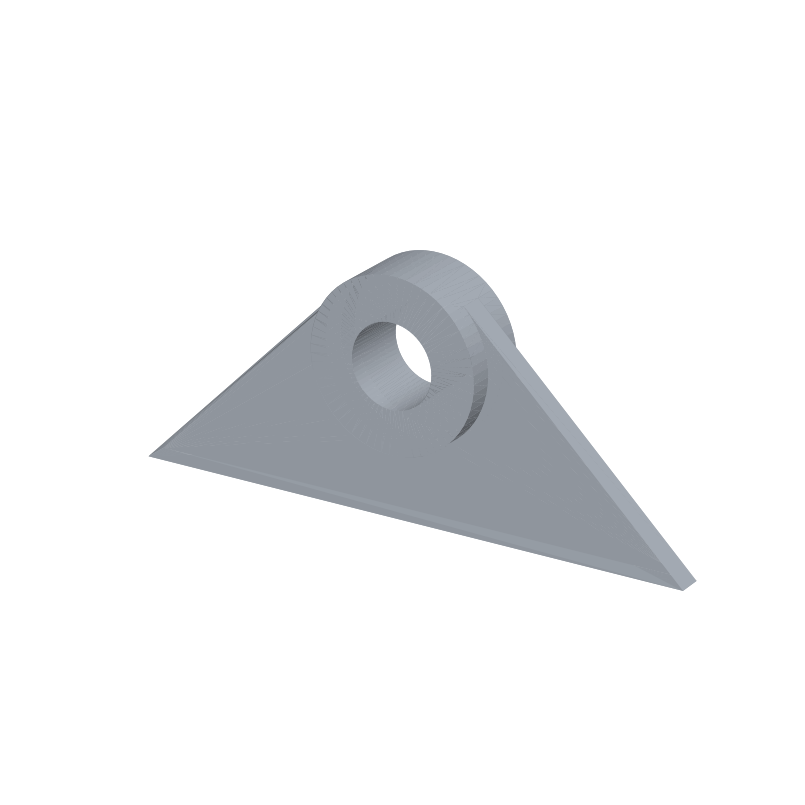
\includegraphics[width=0.62\textwidth]{images/padeye-model.png}
\caption{Lightest case-study padeye, with cheek plates, built by the engine}
\label{fig:padeye-model}
\end{figure}

\subsection{Loads}

The user gives the lifted mass $m$, the number of lifting points, the sling
angle $\theta$ from the horizontal and, if needed, a dynamic factor and the
number of points assumed to carry the load. The force on one padeye follows
from statics.
\begin{align}
V &= \frac{m g \,\text{DAF}}{n_c}, & F &= \frac{V}{\sin\theta}, &
H &= F\cos\theta, & Q &= kF
\label{eq:padeye-loads}
\end{align}
Here $g = 9.80665$~m/s$^2$, DAF is the dynamic factor (default 1.0), $n_c$ is
the number of points carrying the load (default all of them), $V$ and $H$ are
the vertical and in-plane horizontal parts of the sling force $F$, and $Q$ is a
sideways allowance out of the plane of the padeye, with $k = 0.05$ by default.
The sling angle is limited to between 15$^\circ$ and 90$^\circ$. In a simple
lift the plate lies in the plane of its sling.

\subsection{Oblique slings}
\label{sec:oblique-sling}

A padeye fixed to a deck or a structure does not always face its sling. An
oblique sling needs two angles to describe it: the sling angle $\theta$ from
the horizontal, and a second angle $\beta$ between the sling and the plate of
the padeye seen from above. $\beta$ is an advanced setting with a default of
0$^\circ$, the usual case, in which Equation~\eqref{eq:padeye-loads} applies
unchanged. For $\beta > 0$ the sling force is split into
\begin{equation}
H = F\cos\theta\cos\beta, \qquad
Q = F\max(\cos\theta\sin\beta,\; k), \qquad
\gamma = \sin^{-1}(\cos\theta\sin\beta)
\label{eq:oblique}
\end{equation}
where $Q$ is the larger of the real sideways part and the allowance $kF$, and
$\gamma$ is the angle between the sling and the plane of the plate. The base,
shear and weld checks use these $H$ and $Q$. The head checks keep the full
sling force $F$, which is conservative because only $F\cos\gamma$ acts in the
plane of the plate. The finite element model applies the in-plane part
$\sqrt{H^2 + V^2}$ through the hole and $Q$ across it.

The shackle can swing about its pin in the plane of the padeye, but it cannot
swing out of that plane, so $\gamma$ is the side-load angle of the shackle.
Crosby rates screw-pin and bolt-type shackles loaded at an angle to their
in-line axis at a share $r(\gamma)$ of the working load limit
\cite{crosbySideLoad}: 100\% up to 10$^\circ$, 85\% to 20$^\circ$, 75\% to
30$^\circ$, 70\% to 45$^\circ$, 60\% to 55$^\circ$, 55\% to 70$^\circ$ and 50\%
to 90$^\circ$. Shackles larger than 3~in keep the full rating only to
5$^\circ$, 85\% to 10$^\circ$, and need a separate analysis beyond that, which
\NEMO{} treats as not allowed. The shackle is chosen, and the shackle rating is
checked, against $r(\gamma)\,\text{WLL}$.

\subsection{Checks to ASME BTH-1}

The head checks follow the pin-connected plate provisions of ASME BTH-1
\cite{asmeBTH1}. Because the head is a circle concentric with the hole, the
edge distance $R$ and the net width $b_e = R - D_h/2$ are the same in every
in-plane direction. The head checks therefore use the full sling force $F$ for
any sling angle. With cheek plates, the smaller of $R$ and $R_c$ and the lower
yield of the two plates are used. $F_y$ and $F_u$ are the minimum yield and
tensile strengths for the plate thickness and $D_p$ is the shackle pin
diameter.
\begin{align}
C_r &= 1 - 0.275\sqrt{1 - D_p^2/D_h^2}
\label{eq:cr}\\
b_\text{eff} &= \min\!\left(b_e,\; 4t,\; 0.6\,\frac{F_u}{F_y}\sqrt{\frac{D_h}{b_e}}\; b_e\right)
\label{eq:beff}\\
P_t &= \frac{C_r F_u \, 2 t \, b_\text{eff}}{1.20 N_d}
\label{eq:pt}\\
P_b &= \frac{C_r F_u}{1.20 N_d}\left[1.13\left(R - \frac{D_h}{2}\right) + \frac{0.92\, b_e}{1 + b_e/D_h}\right] t
\label{eq:pb}\\
P_v &= \frac{0.70 F_u A_v}{1.20 N_d}, \qquad
A_v = 2\left[a + \frac{D_p}{2}\left(1 - \cos\phi\right) - Z\right] t
\label{eq:pv}\\
P_p &= \frac{C F_y D_p t}{N_d}
\label{eq:pp}
\end{align}
In Equation~\eqref{eq:pv}, $a = R - D_h/2$, $\phi = 55 D_p/D_h$ in degrees,
and $Z = R - \sqrt{R^2 - (D_p \sin\phi/2)^2}$ is the loss of shear plane at the
curved edge. In Equation~\eqref{eq:pp}, $C = 1.25$ for service class~0 and
$0.63$ for classes 1 to 4. Each capacity is compared with $F$.

The base of the main plate, $L$ by $t_\text{main}$, is checked as a
cantilever of length $h$ under $V$, $H$ and $Q$.
\begin{gather}
f_a = \frac{V}{L t}, \quad
f_{bx} = \frac{H h}{t L^2/6}, \quad
f_{by} = \frac{Q h}{L t^2/6}, \quad
f_v = \frac{\sqrt{H^2 + Q^2}}{L t}
\label{eq:base-stress}\\
\frac{f_a}{F_y/N_d} + \frac{f_{bx}}{F_{bx}} + \frac{f_{by}}{1.25F_y/N_d} \leq 1,
\qquad f_v \leq \frac{F_y}{\sqrt{3}\,N_d}
\label{eq:base-combined}
\end{gather}
The strong-axis allowable $F_{bx}$ includes lateral-torsional buckling of the
plate as a rectangular bar. With $\lambda = h L/t^2$, $F_{bx} = 1.25F_y/N_d$ for
$\lambda \leq 0.08E/F_y$, falls linearly as
$[1.52 - 0.274\lambda F_y/E]F_y/N_d$ up to $\lambda = 1.9E/F_y$, and is
$1.9E/(\lambda N_d)$ beyond that.

The fillet welds are checked on the throat against
$F_w = 0.60E_{xx}/(1.20N_d)$, with $E_{xx} = 482$~MPa for E70XX electrodes.
The base weld is two fillet lines of length $L$ with throat $a = 0.707w$ for
leg $w$, their centrelines $t_\text{main} + a$ apart. The normal stress from
$V$, $Hh$ and $Qh$ on this weld group and the shear from $\sqrt{H^2+Q^2}$ are
combined as a vector resultant on the throat. Each cheek plate carries
$F t_c/t$ through one fillet around its circumference $2\pi R_c$.

\subsection{Practice checks}

Some needs of a padeye are not covered by BTH-1. They are checked as
\NEMO{} practice and labelled so in the reports
(Table~\ref{tab:padeye-practice}).

\begin{table}[H]
\centering
\caption{Padeye checks taken from practice and catalogue data}
\label{tab:padeye-practice}
\small
\begin{tabularx}{\textwidth}{lXl}
\toprule
\textbf{Check} & \textbf{Rule} & \textbf{Severity}\\
\midrule
Hole clearance & $D_h \geq D_p + 1$~mm & Required\\
Shackle fit & $t + 2$~mm $\leq$ jaw width & Required\\
Shackle rating & $F/g \leq r(\gamma)\,$WLL, the working load limit reduced for side loading (Section~\ref{sec:oblique-sling}) \cite{crosby2019,crosbySideLoad} & Required\\
Jaw fill & $t \geq 0.6 \times$ jaw width, so the shackle cannot tilt on the pin & Advice\\
Pin fit & $D_p/D_h \geq 0.90$, after the BTH-1 commentary on clearance & Advice\\
Minimum fillet size & AWS D1.1 minimum for the thicker part joined \cite{awsD11} & Advice\\
\bottomrule
\end{tabularx}
\end{table}

\section{Pipe support bracket model}
\label{sec:bracket-model}

\subsection{Geometry}

The bracket is a horizontal seat plate, $L \times b \times t_s$, welded to a
bulkhead and stiffened by two triangular knees of thickness $t_k$
(Figure~\ref{fig:bracket-model}). The knees are flush with the seat edges,
$h_k$ deep at the bulkhead and run out to the seat tip. The pipe sits on the
seat at $e = \text{gap} + \text{insulation} + D/2$ from the bulkhead, held by
a U-bolt of diameter $d$ whose legs pass through holes of $d + 2$~mm at
$x = e \pm (D+d)/2$. The seat length is
$L = e + (D+d)/2 + 1.5d_\text{hole}$, rounded up to 5~mm.

\begin{figure}[H]
\centering
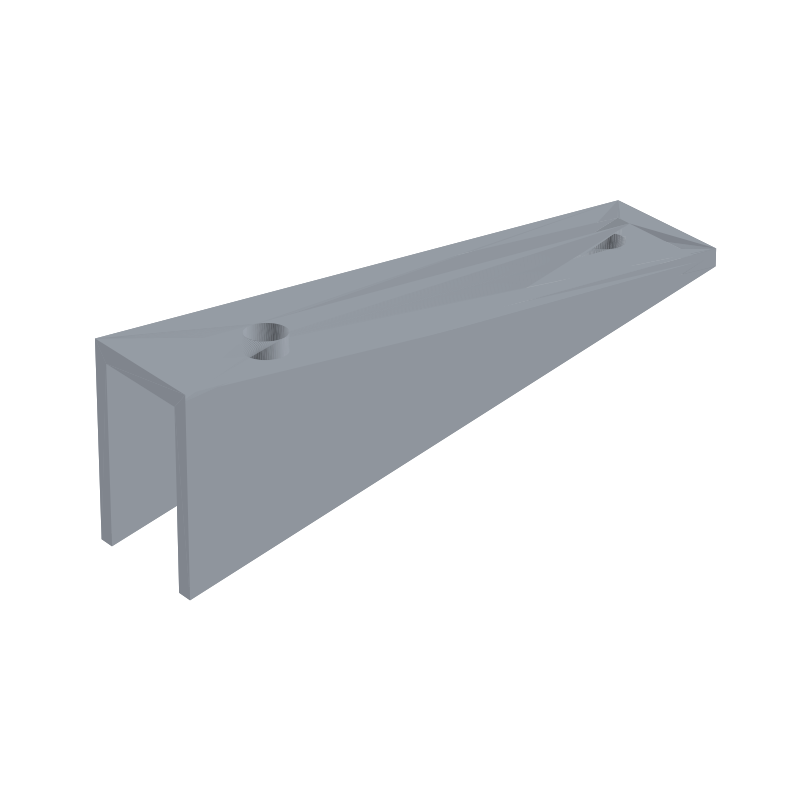
\includegraphics[width=0.6\textwidth]{images/bracket-model.png}
\caption{Lightest case-study pipe support bracket, for an NPS~4 seawater line}
\label{fig:bracket-model}
\end{figure}

\subsection{Loads}

The weight per metre of pipe is $q = g(m_\text{pipe} + m_\text{contents} +
m_\text{insulation})$, with the pipe metal and the bore from ASME B36.10M. One
bracket carries
\begin{equation}
W = k_c\, q\, S
\label{eq:bracket-weight}
\end{equation}
where $S$ is the support spacing and $k_c$ the continuity factor. The default
$k_c = 1.25$ is the middle-support reaction of a two-span continuous beam. Ship
motion adds inertia. The design forces at the pipe are
\begin{equation}
F_z = W(1 + a_v), \quad
F_u = W(a_v - 1) \text{ when } a_v > 1, \quad
F_x = W a_h, \quad
F_y = \mu F_z
\label{eq:bracket-loads}
\end{equation}
for downward, upward, across-pipe and along-pipe directions. The horizontal
acceleration $a_h$ is the athwartships value for a fore-and-aft pipe and the
fore-and-aft value otherwise. Friction $\mu$ (default 0.3) sets the along-pipe
force. The accelerations are inputs. \NEMO{} does not compute them from a
classification society method.

\subsection{Checks to AISC 360-16}

The structural checks use AISC 360-16 in allowable strength design
\cite{aisc2016}. Table~\ref{tab:bracket-checks} lists them. The arm is checked
at 61 stations between the bulkhead and the pipe. At each station the section
is the seat flange plus the two knee webs of depth $h_k(1 - x/L)$. The bending
allowable is taken at first yield, $Z/S = 1$, because the thin knees are not
compact.

\begin{table}[H]
\centering
\caption{Bracket checks}
\label{tab:bracket-checks}
\small
\begin{tabularx}{\textwidth}{>{\raggedright\arraybackslash}p{0.22\textwidth}X}
\toprule
\textbf{Check} & \textbf{Method}\\
\midrule
Arm bending & $U(x) = \dfrac{F_x}{A F_t} + \dfrac{M_y}{S_\text{min} F_b} + \dfrac{M_z}{S_z F_b}$ with $M_y = F_z(e-x) + F_x(D/2 - \bar z)$ and $M_z = F_y(e-x)$; the maximum over the stations (Chapter~H)\\
Arm shear & $V/(2t_k h(x) + b t_s)$ against $0.6F_y/\Omega$ (Chapter~G)\\
Welds to the bulkhead & Line-weld group of two lines across the seat and two per knee. $f_n = N/A_w + M_y c/I_w + M_z(b/2)/I_{wz}$, $f_s = \sqrt{V^2 + F_y^2}/A_w$, resultant on the throat (J2.4)\\
Knee-to-seat welds & Shear flow $VQ/I_y$ at the root over four fillets\\
Seat between the knees & A strip of width $\min(L, b - t_k)$ spanning $l = b - t_k$, $M = \max(F_z l/8,\; T l/4)$, against $1.5F_y/\Omega$ (F11)\\
U-bolt & $T = F_u/2 + F_x(D/2)/s$ per leg and $V = F_x/2$, with $(f_t/F_t)^2 + (f_v/F_v)^2 \leq 1$ (J3.6, J3.7)\\
Deflection & $\delta = \int F_z(e-x)^2/(EI(x))\,dx + \int F_z/(GA_v(x))\,dx$ by Simpson's rule, against a limit set for the job (1~mm by default)\\
Knee free edge (advice) & $l_e \leq 50t_k\sqrt{235/F_y}$, after ship-structure bracket rules\\
Pipe on its brackets (advanced, on by default) & Dunkerley's combined frequency of the span and the bracket at least the margin from every excitation (Section~\ref{sec:bracket-flexibility})\\
\bottomrule
\end{tabularx}
\end{table}

The smallest U-bolt that passes is used, but not less than M10 for pipes under
60~mm outside diameter, M12 under 170~mm, M16 under 280~mm and M20 above. This
is \NEMO{} practice so that a small load does not lead to a U-bolt too slender
to handle.

\subsection{Pipe span checks}
\label{sec:pipe-span}

A bracket can be strong enough while the pipe between two brackets still
fails, most often by resonating with the machinery. \NEMO{} checks the span
as well as the bracket. The first natural frequency of a simply supported
span is
\begin{equation}
f_n = \frac{\pi}{2}\sqrt{\frac{EI}{m S^4}}
\label{eq:span-frequency}
\end{equation}
with $m$ the mass per metre of pipe, contents and insulation. The excitation
frequencies come from the machinery data in the job.
\begin{gather}
f_\text{shaft} = \frac{n_p}{60}, \quad
f_\text{blade} = Z\frac{n_p}{60}, \quad
f_{2\,\text{blade}} = 2Z\frac{n_p}{60}, \quad
f_\text{engine} = \frac{n_e}{60}, \quad
f_\text{firing} = \frac{c\, n_e}{60\,s}
\label{eq:excitations}
\end{gather}
Here $n_p$ and $n_e$ are the propeller and engine speeds in rpm, $Z$ the
number of blades, $c$ the number of cylinders, and $s = 2$ for a four-stroke
engine and 1 for a two-stroke. The span passes when $f_n$ is at least a
margin, 20\% by default, away from every excitation.

Two further checks limit pipe stress and sag. The bending stress
$\sigma = q_d S^2/(10Z)$ uses $q_d = q\sqrt{(1+a_v)^2 + a_h^2}$ and is
compared with $F_{y,\text{pipe}}/1.67$. The sag $5qS^4/(384EI)$ is advised to
stay under 2.5~mm, the figure used in MSS SP-58 style span tables
\cite{mssSP58}. Finally, \NEMO{} reports a recommended maximum spacing, the
smallest of the spans that meet the stress limit, the sag limit and
$f_n \geq (1 + \text{margin})$ times the highest excitation.

Span checks have their own category. The sizing search ignores them, because
the size of the bracket cannot change them, but a failing required span check
still fails the design and is shown first in the results.

\subsection{Bracket flexibility}
\label{sec:bracket-flexibility}

Equation~\eqref{eq:span-frequency} treats the supports as rigid. A real
bracket bends a little under the pipe, and the pipe then vibrates on springs,
at a lower frequency. This is an advanced setting that is on by default,
because it needs no further input. The bracket's stiffness under the pipe and
the pipe mass it carries give it its own frequency, and Dunkerley's method
\cite{blevins1979} combines the two:
\begin{equation}
k = \frac{F_z}{\delta}, \qquad
f_b = \frac{1}{2\pi}\sqrt{\frac{k\,g}{W}}, \qquad
\frac{1}{f^2} = \frac{1}{f_n^2} + \frac{1}{f_b^2}
\label{eq:dunkerley}
\end{equation}
with $\delta$ the deflection of the bracket at the pipe under $F_z$
(Table~\ref{tab:bracket-checks}) and $W$ the static weight on one bracket.
Dunkerley's estimate errs low, which is on the safe side when the span is
meant to stay above the excitations. The combined frequency $f$ must keep the
same margin from every excitation. Unlike the span checks, this one depends on
the bracket, so it is placed in the stiffness category and the sizing search
stiffens the bracket if it fails. When the span already fails on rigid
supports, no bracket can fix it, and the check moves to the span category.

\section{Stabilizer fin model}
\label{sec:fin-model}

\subsection{Geometry}

The fin is a rectangular foil of span $b$ and chord $c$ with a symmetric
NACA four-digit section of thickness ratio $t/c$. Its internal structure is a
plated skin, a front and a rear spar at fixed chord fractions, ribs at a
uniform pitch and a solid stock at chord fraction $x_s/c$ that turns the fin
and carries its load into the bearings in the hull
(Figure~\ref{fig:fin-model}). The ribs follow the inside of the skin.

\begin{figure}[H]
\centering
\begin{subfigure}{0.48\textwidth}
\centering
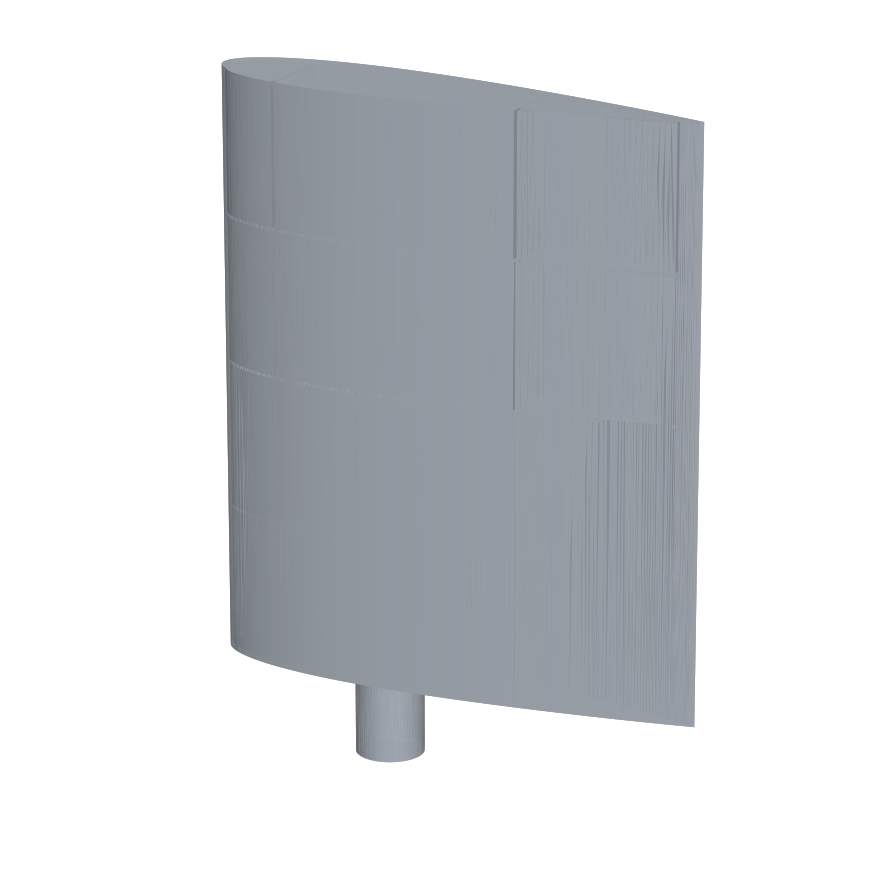
\includegraphics[width=\textwidth]{images/fin-model.png}
\caption{Outside of the fin and the stock}
\end{subfigure}
\hfill
\begin{subfigure}{0.48\textwidth}
\centering
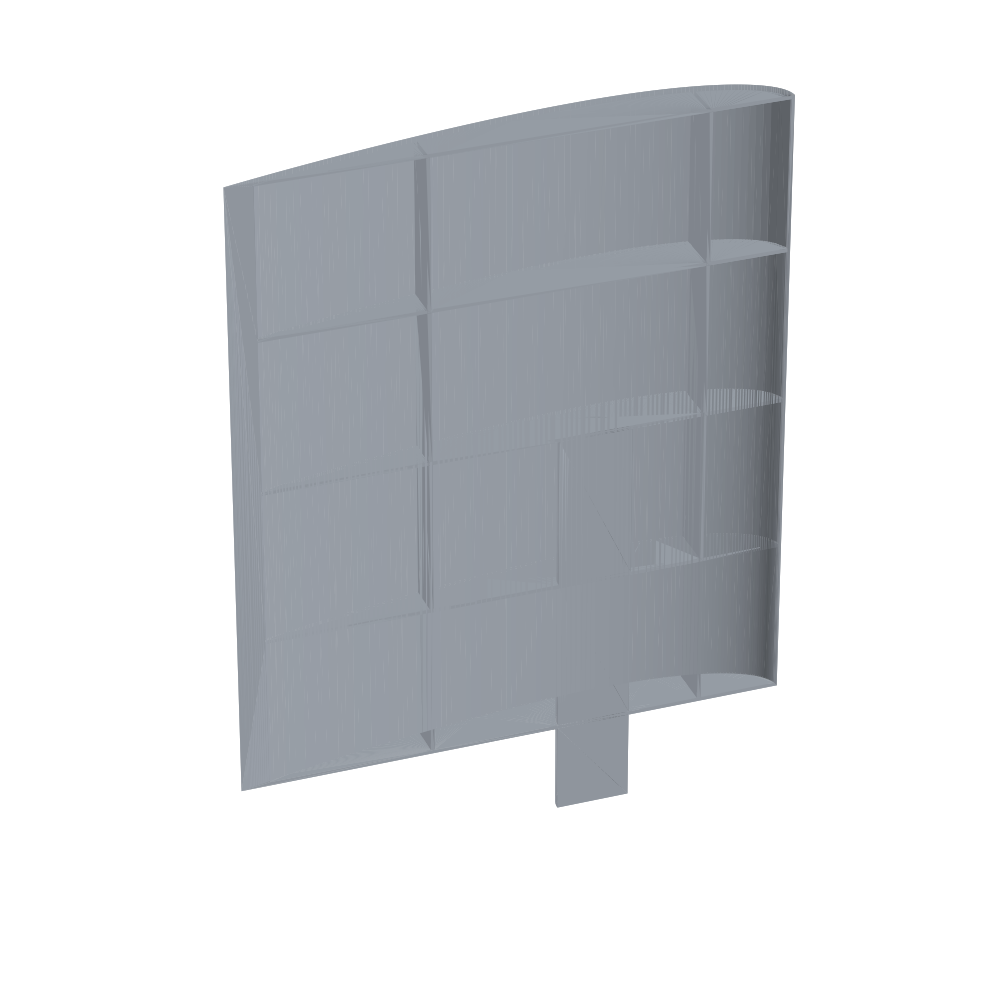
\includegraphics[width=\textwidth]{images/fin-cutaway.png}
\caption{Skin removed to show spars, ribs and stock}
\end{subfigure}
\caption{Lightest case-study stabilizer fin built by the engine}
\label{fig:fin-model}
\end{figure}

\subsection{Loads from two methods}

The fin load is derived twice, by a foil model and by the rule formula, and the
larger is used. This answers requirement R4 and guards against either method
being unconservative for an unusual fin.

The foil model treats the fin as a low-aspect-ratio wing next to the hull. The
hull acts as a mirror plane, so the effective aspect ratio is $A_e = 2b/c$.
Following Whicker and Fehlner \cite{whicker1958}, as used for rudders by
Molland and Turnock \cite{molland2007},
\begin{gather}
\frac{dC_L}{d\alpha} = \frac{0.9 \cdot 2\pi A_e}{\sqrt{A_e^2 + 4} + 1.8},
\qquad
C_L = \frac{dC_L}{d\alpha}\,\alpha + \frac{C_{Dc}}{A_e}\,\alpha^2
\label{eq:whicker}\\
L = \tfrac{1}{2}\rho V^2 A\, C_L
\label{eq:lift}
\end{gather}
where $\alpha$ is the largest fin angle in radians, $C_{Dc} = 0.8$ is the
cross-flow drag coefficient for a square tip, $A = bc$ and
$\rho = 1025$~kg/m$^3$. The second term of $C_L$ is the non-linear lift that a
low-aspect-ratio foil develops at large angles.

The rule formula is the rudder force of IACS UR S10 \cite{iacsS10},
\begin{equation}
C_R = K_1 K_2 K_3 \, 132\, A V^2
\label{eq:ur-force}
\end{equation}
in newtons with $V$ in knots, $K_1 = (\lambda + 2)/3$ with $\lambda = b^2/A$
limited to 2, $K_2 = 1.10$ for a NACA section and $K_3 = 0.8$ for a foil
outside the propeller jet. The design force is $F = \max(L, C_R)$.

The twisting moment on the stock is $Q = F c\,|0.33 - x_s/c|$, at least
$0.1Fc$. The force is taken to act at mid-span, so the bending moment at the
fin root is $M_r = 0.5Fb$ and at the outer bearing
$M_s = F(0.5b + l_g)$, with $l_g$ the gap between the fin root and the
bearing.

\subsection{Astern condition}
\label{sec:astern}

UR S10 requires the rudder force and torque for the astern condition as well
as ahead \cite{iacsS10}. \NEMO{} includes it by default; it needs no input
because the rule sets the least astern speed. With $V_a$ the astern speed, not
less than $0.5V$, $K_2 = 0.80$ for a NACA section astern (UR S10 Table~1), and
the centre of pressure moved aft to 0.66 of the chord (S10.2.1.2),
\begin{equation}
C_{Ra} = K_1 K_2 K_3\,132\,A V_a^2, \qquad
Q_a = C_{Ra}\,c\,|0.66 - x_s/c|, \qquad
M_{sa} = C_{Ra}(0.5b + l_g)
\label{eq:astern}
\end{equation}
The astern force is much smaller than the ahead force, but its lever about
the stock is larger, so for a stock placed well forward the astern twist can
exceed the ahead twist. The stock checks are made for both conditions and
report the worse one. The user can enter a higher astern speed, or switch the
condition off for a fin that is always centred and locked astern.

\subsection{Stock bearings}
\label{sec:bearings}

The stock passes through two bearings in the hull: an outer bearing at
$l_g$ from the fin root and an inner bearing $l$ further in. Sizing them is an
advanced setting, off by default, because $l$ and the bearing material are
often not known at the first design stage. With $a = 0.5b + l_g$ the lever from
the outer bearing to the fin force, the bearing reactions are
\begin{equation}
P_1 = F\,\frac{a + l}{l}, \qquad P_2 = F\,\frac{a}{l}
\label{eq:bearings}
\end{equation}
UR S10.8.2 requires a projected bearing area of at least $P/q_a$, with the
allowable surface pressure $q_a$ from its Table~3: 2.5~N/mm$^2$ for lignum
vitae, 4.5 for white metal, 5.5 for synthetic material harder than 60 Shore~D,
and 7.0 for steel or bronze. The bearing diameter $d_b$ is the stock plus two
liners of the least thickness in S10.8.1, 8~mm (22~mm for lignum). The least
bearing length is then $L = P/(q_a d_b)$, and S10.8.3 limits it to
$1.2\,d_b$. If the length would exceed that, the stock is made larger, which
widens the bearing. The working also gives the least bearing clearance on the
diameter from S10.8.4.

\subsection{Panel method for pressure and cavitation}

The lift formula gives the force but not the pressure on the foil, and
cavitation depends on the lowest pressure. \NEMO{} solves the section with the
Hess-Smith panel method \cite{hess1967}. The section outline is divided into
160 panels with cosine spacing, each carrying a constant source strength, with
one vortex strength shared by all panels. The Kutta condition at the trailing
edge closes the system. The section angle that gives the fin's lift
coefficient is found by solving for the two-dimensional lift slope, and the
pressure distribution at that angle gives $C_{p,\text{min}}$. Cavitation is
flagged when
\begin{equation}
-C_{p,\text{min}} > \sigma = \frac{p_a + \rho g h - p_v}{\tfrac{1}{2}\rho V^2}
\label{eq:cavitation}
\end{equation}
with $p_a = 101.3$~kPa the atmospheric pressure, $h$ the depth of the fin
below the surface and $p_v = 1.7$~kPa the vapour pressure of sea water at
about 15$^\circ$C. This is an advice check.
An inviscid panel method cannot model separated or cavitating flow, so the
check warns of cavitation onset and does not predict its extent.

\subsection{Structural checks}

The fin body between the spars is treated as a box girder. Its second moment
of area is $I = 2\int t y^2\, ds + t_w(h_f^3 + h_r^3)/12$, where the integral
runs along the skin between the spars and $h_f$ and $h_r$ are the spar depths.
The checks are listed in Table~\ref{tab:fin-checks}. The stress limits of UR
S10 are given as multiples of $1/k$.

\begin{table}[H]
\centering
\caption{Stabilizer fin checks}
\label{tab:fin-checks}
\small
\begin{tabularx}{\textwidth}{>{\raggedright\arraybackslash}p{0.22\textwidth}X}
\toprule
\textbf{Check} & \textbf{Method}\\
\midrule
Stock torsion & $\tau_t = 5.1Q/D^3 \times 10^3 \leq 68/k$ (S10.4.1), ahead and astern\\
Stock combined & $\sigma_b = 10.2M_s/D^3 \times 10^3$, $\sigma_e = \sqrt{\sigma_b^2 + 3\tau_t^2} \leq 118/k$ (S10.4.2), ahead and astern\\
Stock bearings (advanced) & $L = P/(q_a d_b) \leq 1.2\,d_b$ for the outer and inner bearing (S10.8.2, 8.3)\\
Stock fit & The stock diameter is less than the foil thickness at the stock position (practice)\\
Fin body bending & $\sigma_b = M_r y/I \leq 110/k$ (S10.5.1)\\
Spar web shear & $F/(t_w\sum h) + q_t/t_w \leq 50/k$, with Bredt shear flow $q_t = Q/(2A_\text{box})$ (S10.5.1)\\
Skin combined & $\sigma_e \leq 120/k$ (S10.5.1)\\
Skin plating & $t \geq 5.5\, s\beta\sqrt{(T + C_R 10^{-4}/A)k} + 2.5$ (S10.5.2)\\
Web thickness & $t_w \geq \max(0.7t, 8~\text{mm})$ (S10.5.2)\\
Skin buckling & $\sigma_E = k_b\pi^2E/[12(1-\nu^2)](t/b_p)^2$ with $k_b = \min_m (m b_p/a_p + a_p/(m b_p))^2$, Johnson-Ostenfeld correction above $F_y/2$, factor 1.5 (practice, after Timoshenko and Gere \cite{timoshenko1961})\\
Tip deflection & Point load at mid-span on a cantilever with the box $I$, against a job limit\\
Cavitation (advice) & $-C_{p,\text{min}} \leq \sigma$\\
\bottomrule
\end{tabularx}
\end{table}

In the plating formula, $s$ is the shorter side of a skin panel bounded by
the ribs and spars, $\beta$ a correction for the panel aspect ratio and $T$
the draught in metres. In the buckling check, $a_p$ is the rib pitch and $b_p$
the spar spacing. The skin and web thicknesses must
come from the plate stock. The stock diameter is not taken from stock lists,
because stocks are forged and turned to size.

\section{Sizing method}
\label{sec:sizing}

\subsection{Problem form}

Each part is sized as a mixed problem. Some variables are discrete because
the yard can only use certain sizes. These are the plate thicknesses from the
ticked stock list, the shackle and U-bolt sizes and the standard weld legs. The rest are
continuous, such as the head radius or the knee depth, but must be rounded to
sizes a workshop can mark out. The objective is the steel mass. The
constraints are the required checks, with strength checks held to a target
maximum use.

\NEMO{} handles the two kinds of variable separately. It enumerates the
discrete choices, and for each combination it sizes the continuous variables
with a bounded Nelder-Mead search \cite{nelder1965,lagarias1998}. Nelder-Mead
needs only the objective value, so it works with checks that have corners,
such as the maximum over 61 stations of the arm, and with designs that switch
governing checks. Figure~\ref{fig:sizing-flow} shows the procedure.

\begin{figure}[H]
\centering
\begin{tikzpicture}[node distance=0.55cm, font=\small, every node/.style={text width=6.2cm}]
\node[startstop] (loads) {Loads from the job description};
\node[process, below=of loads] (discrete) {List discrete combinations\\(plate, cheek or knee, shackle or U-bolt)};
\node[decision, below=of discrete, text width=3.4cm] (bound) {Lower-bound mass $<$ best so far?};
\node[process, below=0.7cm of bound] (nm) {Bounded Nelder-Mead on the continuous variables, three starts};
\node[process, below=of nm] (welds) {Choose the smallest standard welds that pass};
\node[process, below=of welds] (round) {Round to buildable sizes; grow until every check passes};
\node[process, below=of round] (keep) {Keep if lighter than the best so far};
\node[startstop, below=of keep] (out) {Repeat for targets 100\%, 85\%, 70\%};
\node[process, right=1.2cm of bound, text width=2.6cm] (skip) {Skip, and log the reason};
\draw[arrow] (loads) -- (discrete);
\draw[arrow] (discrete) -- (bound);
\draw[arrow] (bound) -- node[left, text width=0.8cm] {yes} (nm);
\draw[arrow] (bound) -- node[above, text width=0.6cm] {no} (skip);
\draw[arrow] (nm) -- (welds);
\draw[arrow] (welds) -- (round);
\draw[arrow] (round) -- (keep);
\draw[arrow] (keep) -- (out);
\draw[arrow] (skip.north) |- ([xshift=1cm]discrete.east) node[pos=0.75, above, text width=2.6cm] {next combination};
\end{tikzpicture}
\caption{Sizing procedure used for every part}
\label{fig:sizing-flow}
\end{figure}

\subsection{Bounded Nelder-Mead search}

The continuous variables are scaled to $[0, 1]$ between bounds that depend on
the combination. For the padeye, the head radius runs from
$D_h/2 + \max(0.25D_h, 5)$ to $D_h/2 + 3D_h + 30$~mm, the base length from
$2R$ to $8R$ and, with cheek plates, the cheek radius from $D_h/2 + 10$~mm to
$R$. For the bracket, the knee depth runs from $0.3L$ to $1.5L$ and the seat
width from $2t_k + 2d + 10$~mm to the larger of $3D$ and that minimum plus
150~mm. Every trial point is clipped to the unit box.

The initial simplex has a step of 0.15 in each scaled variable. The search
uses the standard reflection, expansion, contraction and shrink steps with
coefficients 1, 2, 0.5 and 0.5, and stops when the values and the simplex have
both collapsed, or after 200 iterations for the padeye and 160 for the
bracket. Values are cached, so a repeated point costs nothing. Each
combination is searched from three starting points and the best result kept,
because the feasible region can have several pockets.

Constraints enter through a penalty,
\begin{equation}
\Phi(\mathbf{x}) = m(\mathbf{x})\left[1 + 1000 \sum_i \max(U_i - U_{\text{lim},i},\, 0)^2\right]
\label{eq:penalty}
\end{equation}
summed over the required checks, where $U_{\text{lim},i}$ is the target for
strength checks and 1.0 for the others. A design with a geometric problem,
such as a hole that breaks out of the head, scores $10^9$ and is never kept.
The penalty only guides the search. The design that is finally kept is
re-checked after rounding, and only a design that passes every required check
at the target is accepted.

\subsection{Welds, rounding and pruning}

The search evaluates each trial with a reference weld size. The weld leg is
then set to the smallest standard size, between 3~mm and 20~mm, that passes,
is at least the AWS D1.1 minimum for the thicker part and does not exceed a
practical maximum. The base weld of a padeye is limited to $0.75t_\text{main}$
and a cheek weld to $t_c$.

After the search, the continuous variables are rounded up. For the padeye,
$R$, $R_c$ and $h$ are rounded to 1~mm and $L$ to 5~mm. For the bracket, the
knee depth and seat width are rounded to 5~mm. If the rounded design fails at
the target, it is grown in small steps, 2\% in radius and 3\% in length for
the padeye, and checked again, up to 40 times.

Before a combination is searched, \NEMO{} computes the smallest mass it could
possibly have, for example the padeye with the smallest allowed head and the
shortest base. If that lower bound is already heavier than the best design
found so far, the combination is skipped and the reason is written to the
log. In the bracket case study this pruning skipped 60 of 63 combinations.

\subsection{Fin sizing}

The fin search is exhaustive because its variables are few and its checks
are cheap. For each target, the stock diameter is the smallest 5~mm step that
passes both stock checks, ahead and astern, and, when the bearing check is on,
leaves room for bearings no longer than $1.2\,d_b$. Every pair of skin and web thickness from the stock
list, with webs of at least 8~mm, is then combined with every rib spacing from
150~mm to 1000~mm in 25~mm steps, and the lightest passing fin is kept.

\subsection{Three designs}

The sizing is repeated with strength targets of 100\%, 85\% and 70\% maximum
use. The results are offered as \emph{Lightest}, \emph{Balanced (at least 15\%
spare)} and \emph{Extra margin (at least 30\% spare)}. The targets apply on top
of the code's own safety factors. They let the engineer trade mass against
reserve for uncertain loads, corrosion allowance or future changes without
rerunning the search.

\section{Geometry and output files}
\label{sec:cad}

Each kept design is built as an exact solid with build123d, a Python CAD
library on the OpenCASCADE kernel. The padeye is extruded from its outline,
with the hole cut and the cheek rings added. The bracket is the seat and two
knees, with the U-bolt holes. The fin skin is the NACA outline extruded along
the span, less its inside offset by the skin thickness. The spars, the ribs
and the stock are added to it as solids.

The volume of the solid is compared with the formula the mass came from. The
padeye and the bracket match exactly, which checks the geometry code against
the mass code. The fin's mass uses a thin-wall formula. It takes the skin as
its outer perimeter times its thickness and each rib as the full foil area,
and it counts the stock, spars and ribs again where they overlap. The solid
removes these overlaps, so it is about 3.5\% smaller and the mass formula errs
on the heavy side. The difference is shown on the run screen and in the
report.

From the solid, \NEMO{} writes a STEP file for CAD and fabrication systems and
an STL file for the 3D view. A DXF file gives the cutting profiles of the
plates, the padeye plate and cheeks, the bracket seat and knees, or the fin
ribs, with the hole positions.

\section{Built-in finite element analysis}
\label{sec:fea}

\subsection{Mesh and elements}

The same solid that is written to STEP is meshed with Gmsh \cite{gmsh2009}.
The mesh is refined where the stress is expected to change fastest, around
the hole of the padeye and near the bulkhead for the bracket. The fin stock
is a plain shaft and is meshed uniformly. Each design is meshed three times,
with the element size multiplied by 1.0, 0.7 and 0.5.

The displacement field uses quadratic (P2) tetrahedra in scikit-fem
\cite{skfem2020}, with linear elastic isotropic material. Quadratic elements
are used because linear tetrahedra are too stiff in bending, which matters for
the thin plates of all three parts. The stiffness matrix is assembled by a
vectorised routine that builds all element matrices from the shape-function
gradients with a few array operations. A test confirms that it gives the same
matrix as the scikit-fem reference assembly to within $10^{-12}$.

\subsection{Loads and supports}

Loads are applied as surface tractions defined by a \emph{shape} and a target
resultant. The solver integrates the shape over the loaded faces, then scales
it so that its resultant equals the target. The applied total then matches
the design force used by the checks, whatever the mesh. In the padeye case
study it differed by less than 1~N in each direction. This removes the load
transcription error seen during early exploratory testing (requirement R2).

\begin{itemize}
    \item \textbf{Padeye.} The base face is fixed. The in-plane pin load is a
    cosine pressure $p \propto \max(\cos\alpha, 0)$ on the loaded half of the
    hole surface, with $\alpha$ measured from the sling direction, scaled to
    the in-plane sling force. The sideways force $Q$ is applied as a uniform
    axial traction around the full hole bore so that it introduces no spurious
    twisting moment about the pinhole and matches Autodesk Fusion's Bearing
    Load axial distribution.
    \item \textbf{Bracket.} The faces against the bulkhead are fixed. $F_z$,
    $F_x$ and $F_y$ are uniform tractions on a strip of the seat top under the
    pipe, of width the larger of $D/4$, $2.5t_s$ and 1.5 element sizes.
    \item \textbf{Fin stock.} The model is the stock alone, a solid shaft from
    the outer bearing to $0.6b$, fixed at the bearing face. The fin force and
    the twist are tractions on the stock surface between $0.4b$ and $0.6b$.
    The twist is a load whose force resultant is zero, so it is scaled to its
    target moment instead. On a coarse mesh the scaled twist adds a small net
    force. The force load takes up the part of it along the fin force, and the
    rest is reported with the applied total. In the case study it was 1.2\%
    of the fin force on the coarsest mesh and 0.03\% on the finest.
\end{itemize}

\subsection{Solver}

Below 6,000 unknowns the system is solved directly with SciPy's sparse
solver. Larger systems use conjugate gradients preconditioned by
smoothed-aggregation algebraic multigrid from PyAMG
\cite{pyamg2023,vanek1996}, with the six rigid-body modes as the near-null
space, to a relative residual of $10^{-10}$. If the residual has not fallen
below $10^{-8}$ after 600 iterations, the solver falls back to the direct
method. The residual history is written to the engineering log.

\subsection{Results and acceptance}

The six symmetric Cauchy stress tensor components are evaluated at element
corners, averaged at each vertex, and then combined into the nodal von Mises
stress. Averaging the tensor components before computing von Mises matches
standard finite element post-processors and avoids upward scalar-averaging bias
at geometric transitions. After each solve, \NEMO{} records the following.

\begin{itemize}
    \item \textbf{Force and moment balance}, $|\mathbf{F}_\text{applied} +
    \mathbf{R}|/|\mathbf{F}_\text{applied}|$ and the variational moment
    balance $|\mathbf{M}_\text{applied} +
    \mathbf{M}_R|/|\mathbf{M}_\text{applied}|$, where $\mathbf{R}$ and
    $\mathbf{M}_R$ are the support reaction force and moment. Both must close
    to near zero.
    \item \textbf{Mesh convergence}, the change in the assessed peak stress
    between the two finest meshes. The target is 5\% or less.
    \item \textbf{Assessed peak}, the highest von Mises stress in a stated
    region. Sharp 90$^\circ$ transitions where a fixed face meets a free face,
    and where an unmodeled fillet weld leaves a 90$^\circ$ re-entrant step at
    the outer edge of a padeye cheek plate, carry linear-elastic stress
    singularities that diverge as the mesh is refined. Each part therefore
    reads its peak clear of those singular edges. The assessed region is within
    $R + 1$~mm of the hole axis for the padeye (excluding the 90$^\circ$
    cheek-plate step at $r = R_c$, $|y| = t/2$), at $x \geq 1.5$ times the
    thicker plate for the bracket, and from half a diameter outboard of the
    bearing to the loaded length for the stock.
\end{itemize}

A design passes the finite element check when the assessed peak is below
the yield stress and the meshes have converged. For the bracket and the fin
the peak is also compared with the hand stress at the same place, the seat
bending stress and the stock beam stress respectively. The finite element
analysis confirms the hand checks. It does not replace them, because the code
capacities include effects such as fracture and lateral buckling that a
linear model does not capture.

\begin{figure}[H]
\centering
\begin{subfigure}{0.32\textwidth}
\centering
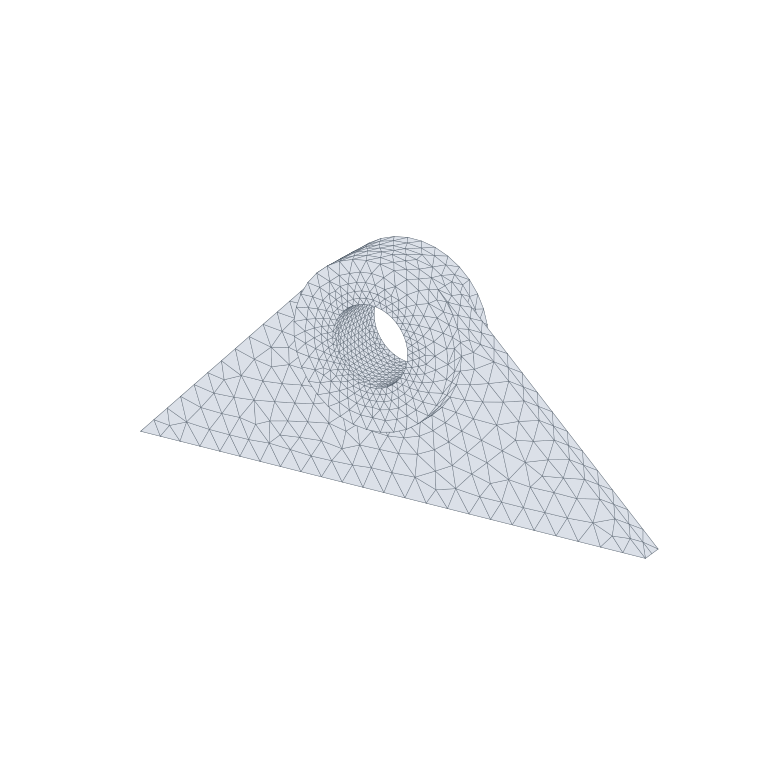
\includegraphics[width=\textwidth]{images/padeye-mesh.png}
\caption{Padeye}
\end{subfigure}
\hfill
\begin{subfigure}{0.32\textwidth}
\centering
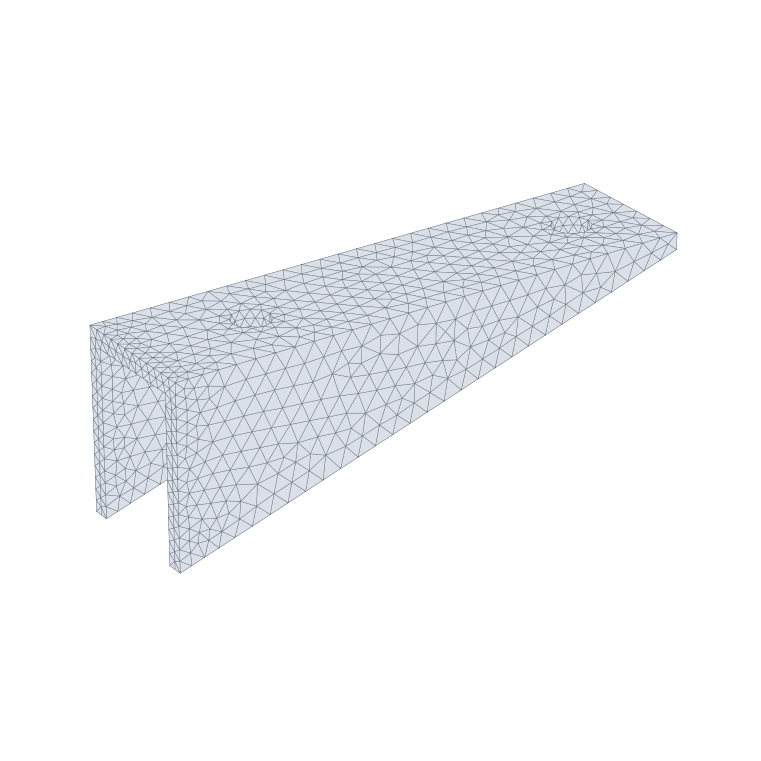
\includegraphics[width=\textwidth]{images/bracket-mesh.png}
\caption{Bracket}
\end{subfigure}
\hfill
\begin{subfigure}{0.32\textwidth}
\centering
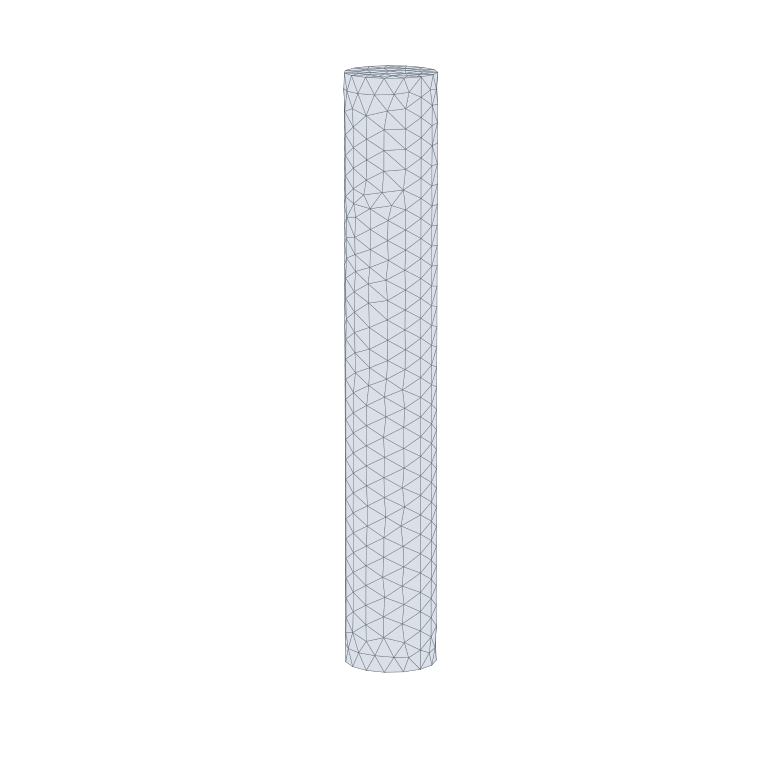
\includegraphics[width=\textwidth]{images/fin-stock-mesh.png}
\caption{Fin stock}
\end{subfigure}
\caption{Finest of the three meshes for each case-study design}
\label{fig:meshes}
\end{figure}

\section{Verification method}
\label{sec:verification-method}

Verification here means checking that the code solves its equations
correctly, as distinct from validation against physical behaviour
\cite{asmeVV10}. Two kinds of evidence were produced.

\textbf{Benchmark suite.} The module \code{nemo.verification} runs the
reference problems in Table~\ref{tab:benchmarks} and reports, for each
quantity, the reference value, the \NEMO{} value, the difference and the
tolerance. The same suite runs from the Verification page of the application,
on the user's own computer, so a checker can confirm the installation they are
using.

\begin{table}[H]
\centering
\caption{Verification benchmarks}
\label{tab:benchmarks}
\small
\begin{tabularx}{\textwidth}{>{\raggedright\arraybackslash}p{0.26\textwidth}>{\raggedright\arraybackslash}X>{\raggedright\arraybackslash}p{0.2\textwidth}}
\toprule
\textbf{Benchmark} & \textbf{What it checks} & \textbf{Reference}\\
\midrule
Padeye hand calculation & Every BTH-1 quantity for a 4~t lift on two points at 60$^\circ$, S355, 20~mm plate, tolerance 0.1\% & Hand calculation in the engineering manual\\
CAD volume & Solid volume of a plain padeye, a padeye with cheeks and a bracket against the exact formula, tolerance 0.01\% & Exact geometry\\
Cantilever & 200 by 20 by 20~mm beam under 1~kN: tip deflection (3\%) and mid-span bending stress (4\%) & Timoshenko beam theory \cite{timoshenko1972}\\
Plate with a hole & 200~mm plate, 20~mm hole, in tension: stress concentration factor, tolerance 5\% & Heywood, in Peterson \cite{peterson2008}\\
Panel method & $C_{p,\text{min}} = -3$ on a circle (0.5\%); lift slope $2\pi(1 + 0.77t/c)$ for NACA~0012 and NACA~0020 (3\%) & Potential flow; Abbott and von Doenhoff \cite{abbott1959}\\
Fin stock & Equivalent stress near the bearing under bending and twist, tolerance 4\% & Beam and torsion theory, as in UR S10.4\\
Support reactions & In every finite element benchmark, the reaction equals the applied load & Statics\\
\bottomrule
\end{tabularx}
\end{table}

\textbf{Automated tests.} The engine has 181 tests in 15 files, run with
pytest after every change. They cover the hand calculation, the behaviour of
the checks when one input changes, CAD volumes for 50 random designs, STEP
export and re-import, the finite element benchmarks, sizing, the working
steps, the run pipeline, the server routes for all three parts, the Fusion
job queue, and each advanced setting against a hand calculation.

\section{Traceability}
\label{sec:traceability}

The tool is meant to be checked by someone who did not write it. Each run
therefore keeps the following records, which answer requirement R9.

\begin{itemize}
    \item \textbf{Working for every check}, as described in
    Section~\ref{sec:check-model}, shown in the application and printed in the
    PDF.
    \item \textbf{Engineering log}, \code{engineering-log.json}, an ordered and
    time-stamped list of events. It records the forces, the shackle or U-bolt choice,
    each search combination and its outcome, thinned samples of designs tried,
    CAD volumes, mesh statistics, solver residual history, force balance and
    mesh convergence. The live run screen of the application is drawn from
    these events as they happen.
    \item \textbf{Every design tried}, \code{designs-evaluated.csv}, with the
    target, discrete choices, dimensions, weld sizes, mass, highest use and
    whether the design met its target.
    \item \textbf{Checksums.} The audit section of the PDF lists the SHA-256
    hash of each run file, so a later change to a file can be detected.
\end{itemize}

The PDF calculation package for each design has a summary page, a
dimensioned drawing, the loads with their working, every check with its
working and source, the finite element results with the mesh study, the
pipe-span or foil results where they apply, the assumptions and limits, and
the audit trail. Examples are shown in Section~\ref{sec:results-package}.

\section{Application and user workflow}
\label{sec:application}

The application is written for an engineer or technician who does not
program. It is installed by double-clicking \code{Install NEMO.bat}. The
installer uses uv to download a private copy of Python~3.12, creates the
engine's environment, installs the libraries, prepares the application and
adds a desktop shortcut. It does not change any other Python on the computer.
\code{Start NEMO.bat} starts the local server and opens the application in the
browser.

The workflow has six screens, in order.

\begin{enumerate}
    \item \textbf{Home} lists the saved projects and starts a new one
    (Figure~\ref{fig:app-home}).
    \item \textbf{New design} asks which part to design.
    \item \textbf{Describe the job} is a form in plain words, such as ``How
    heavy is the load?'' or ``Which plate thicknesses does your workshop
    have?'', with help text and a live 3D preview that updates as values
    change (Figures~\ref{fig:app-describe} and~\ref{fig:app-bracket-motion}). Inputs are validated in the form
    and again by the engine.
    \item \textbf{Assumptions} sets the design basis, with defaults: the rule
    set and, for a padeye, the design category, service class, dynamic factor
    and jaw fill. The bracket and fin have their own versions of this screen.
    Considerations that a simple job does not need sit in a collapsed
    \emph{Advanced settings} section on these screens, with defaults that
    leave a simple job unchanged: the oblique sling angle and load sharing for
    a padeye, the bracket's flexibility in the vibration check, and the fin's
    astern condition and stock bearings.
    \item \textbf{Finding designs} is the live run screen
    (Figure~\ref{fig:app-running}). Each engineering step shows its numbers as
    they are produced, and selecting a step shows its working.
    \item \textbf{Results} shows the three designs, their dimensions, the 3D
    model and stress plot, every check with its working, the engineering
    record and the PDF, and offers the files for download.
\end{enumerate}

A Verification page, reached from the top bar, runs the benchmark suite.
The interface uses one neutral colour scheme with a dark mode and the Inter
typeface. Eleven documents, written in plain language, come with the tool,
including a getting-started guide, a user guide of 1,662 words, an
engineering manual of 3,089 words for checkers, a page each on brackets and
fins, a limits-and-safety page, a glossary and a troubleshooting guide.

\begin{figure}[H]
\centering
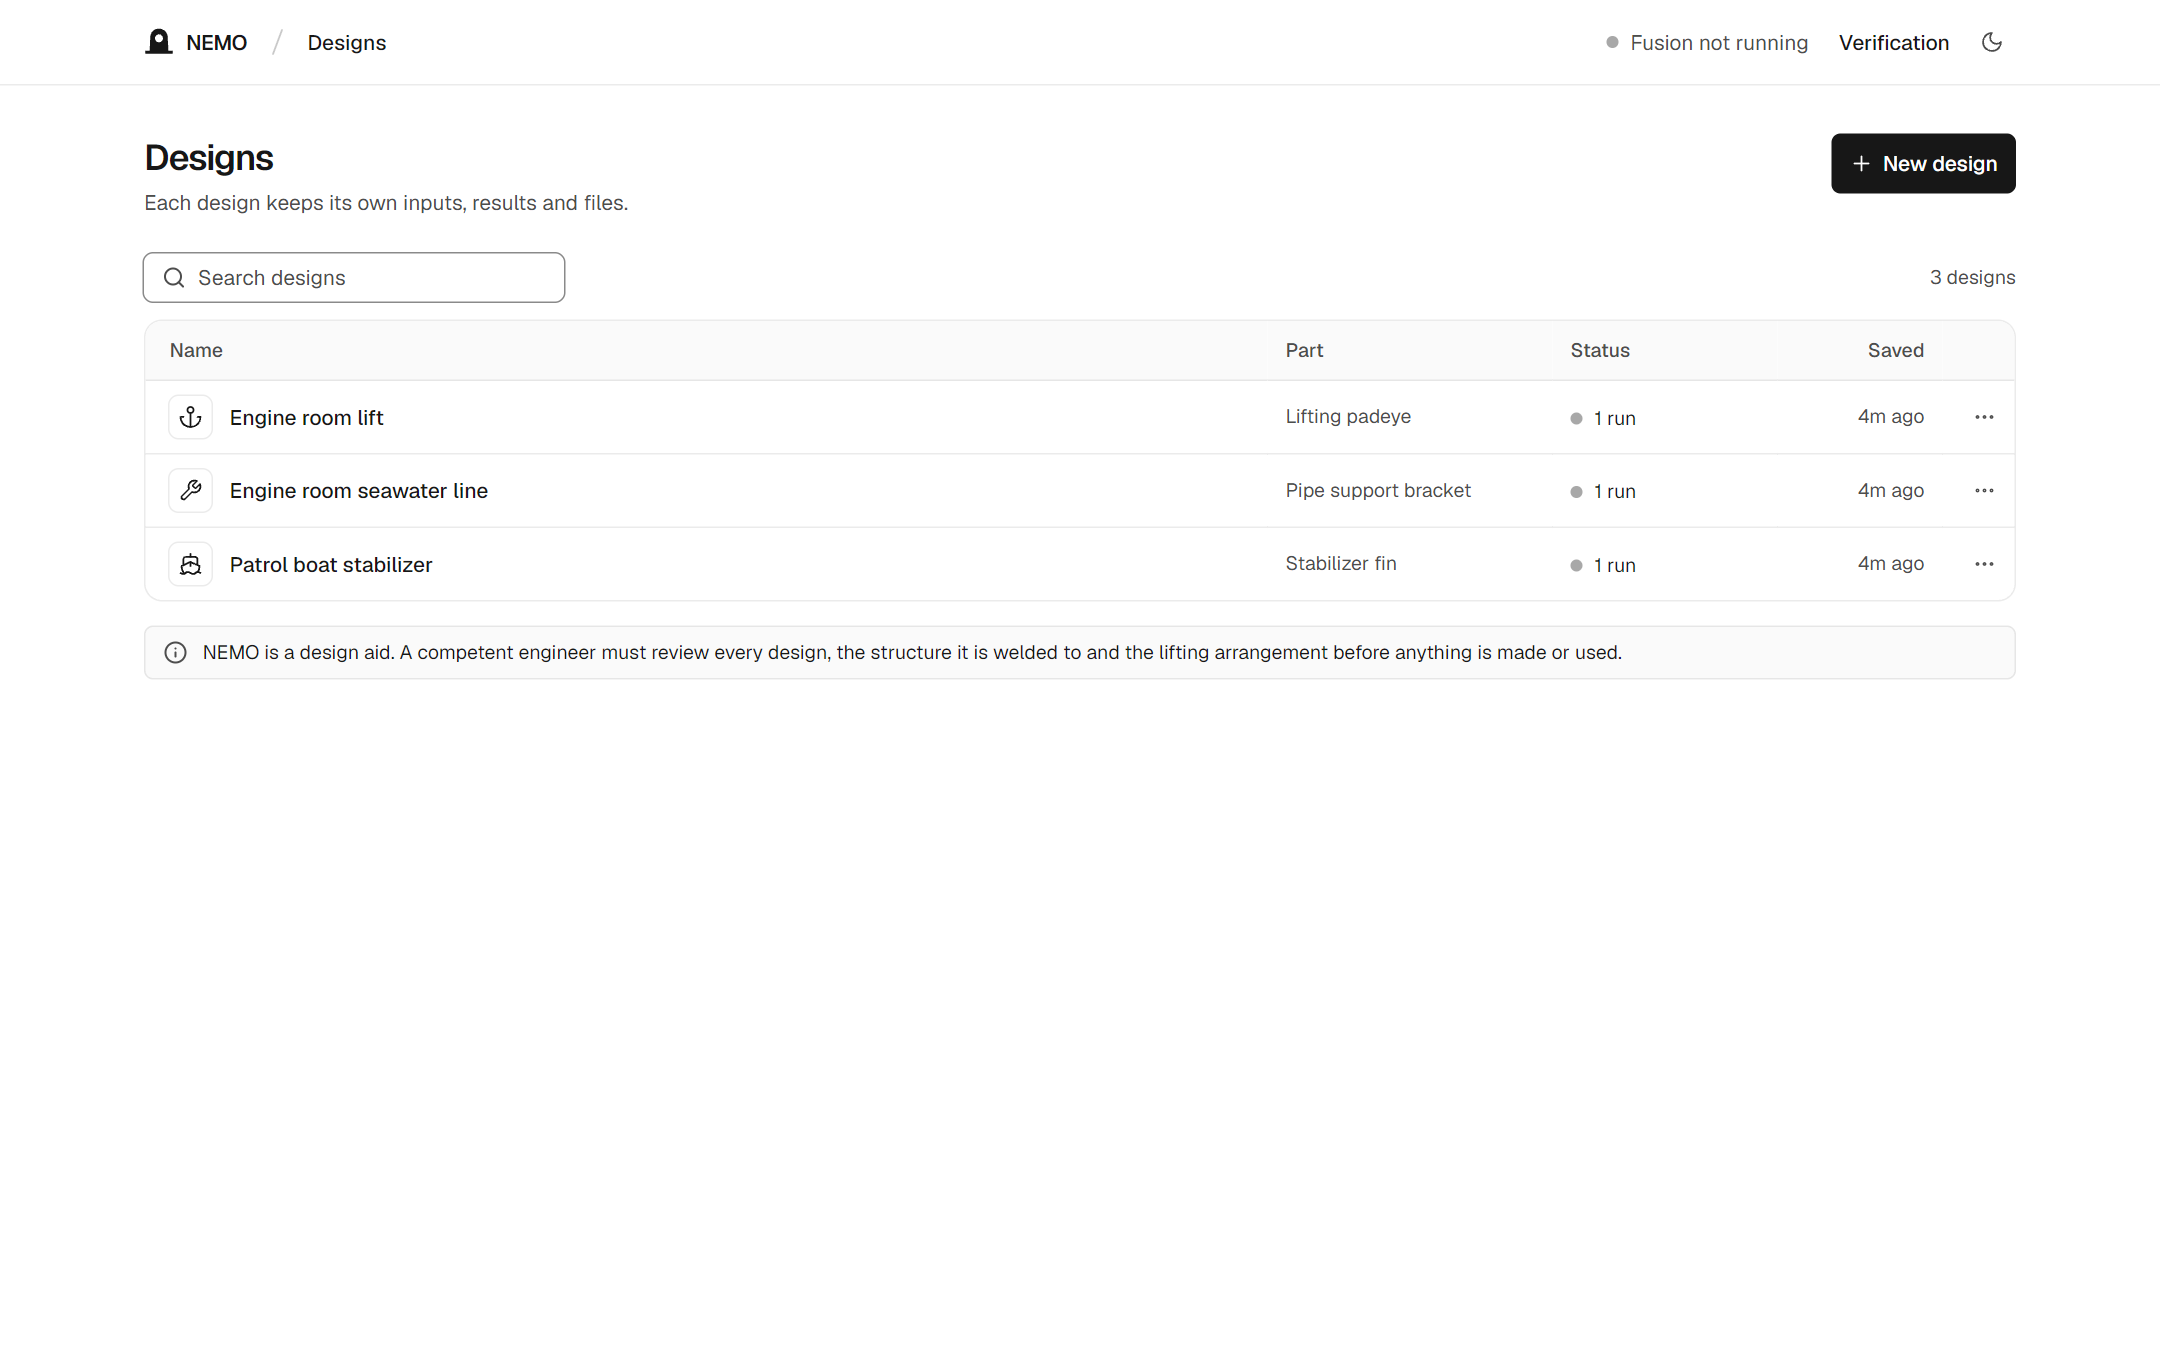
\includegraphics[width=\textwidth]{images/app-home.png}
\caption{Home screen with the three case-study projects}
\label{fig:app-home}
\end{figure}

\begin{figure}[H]
\centering
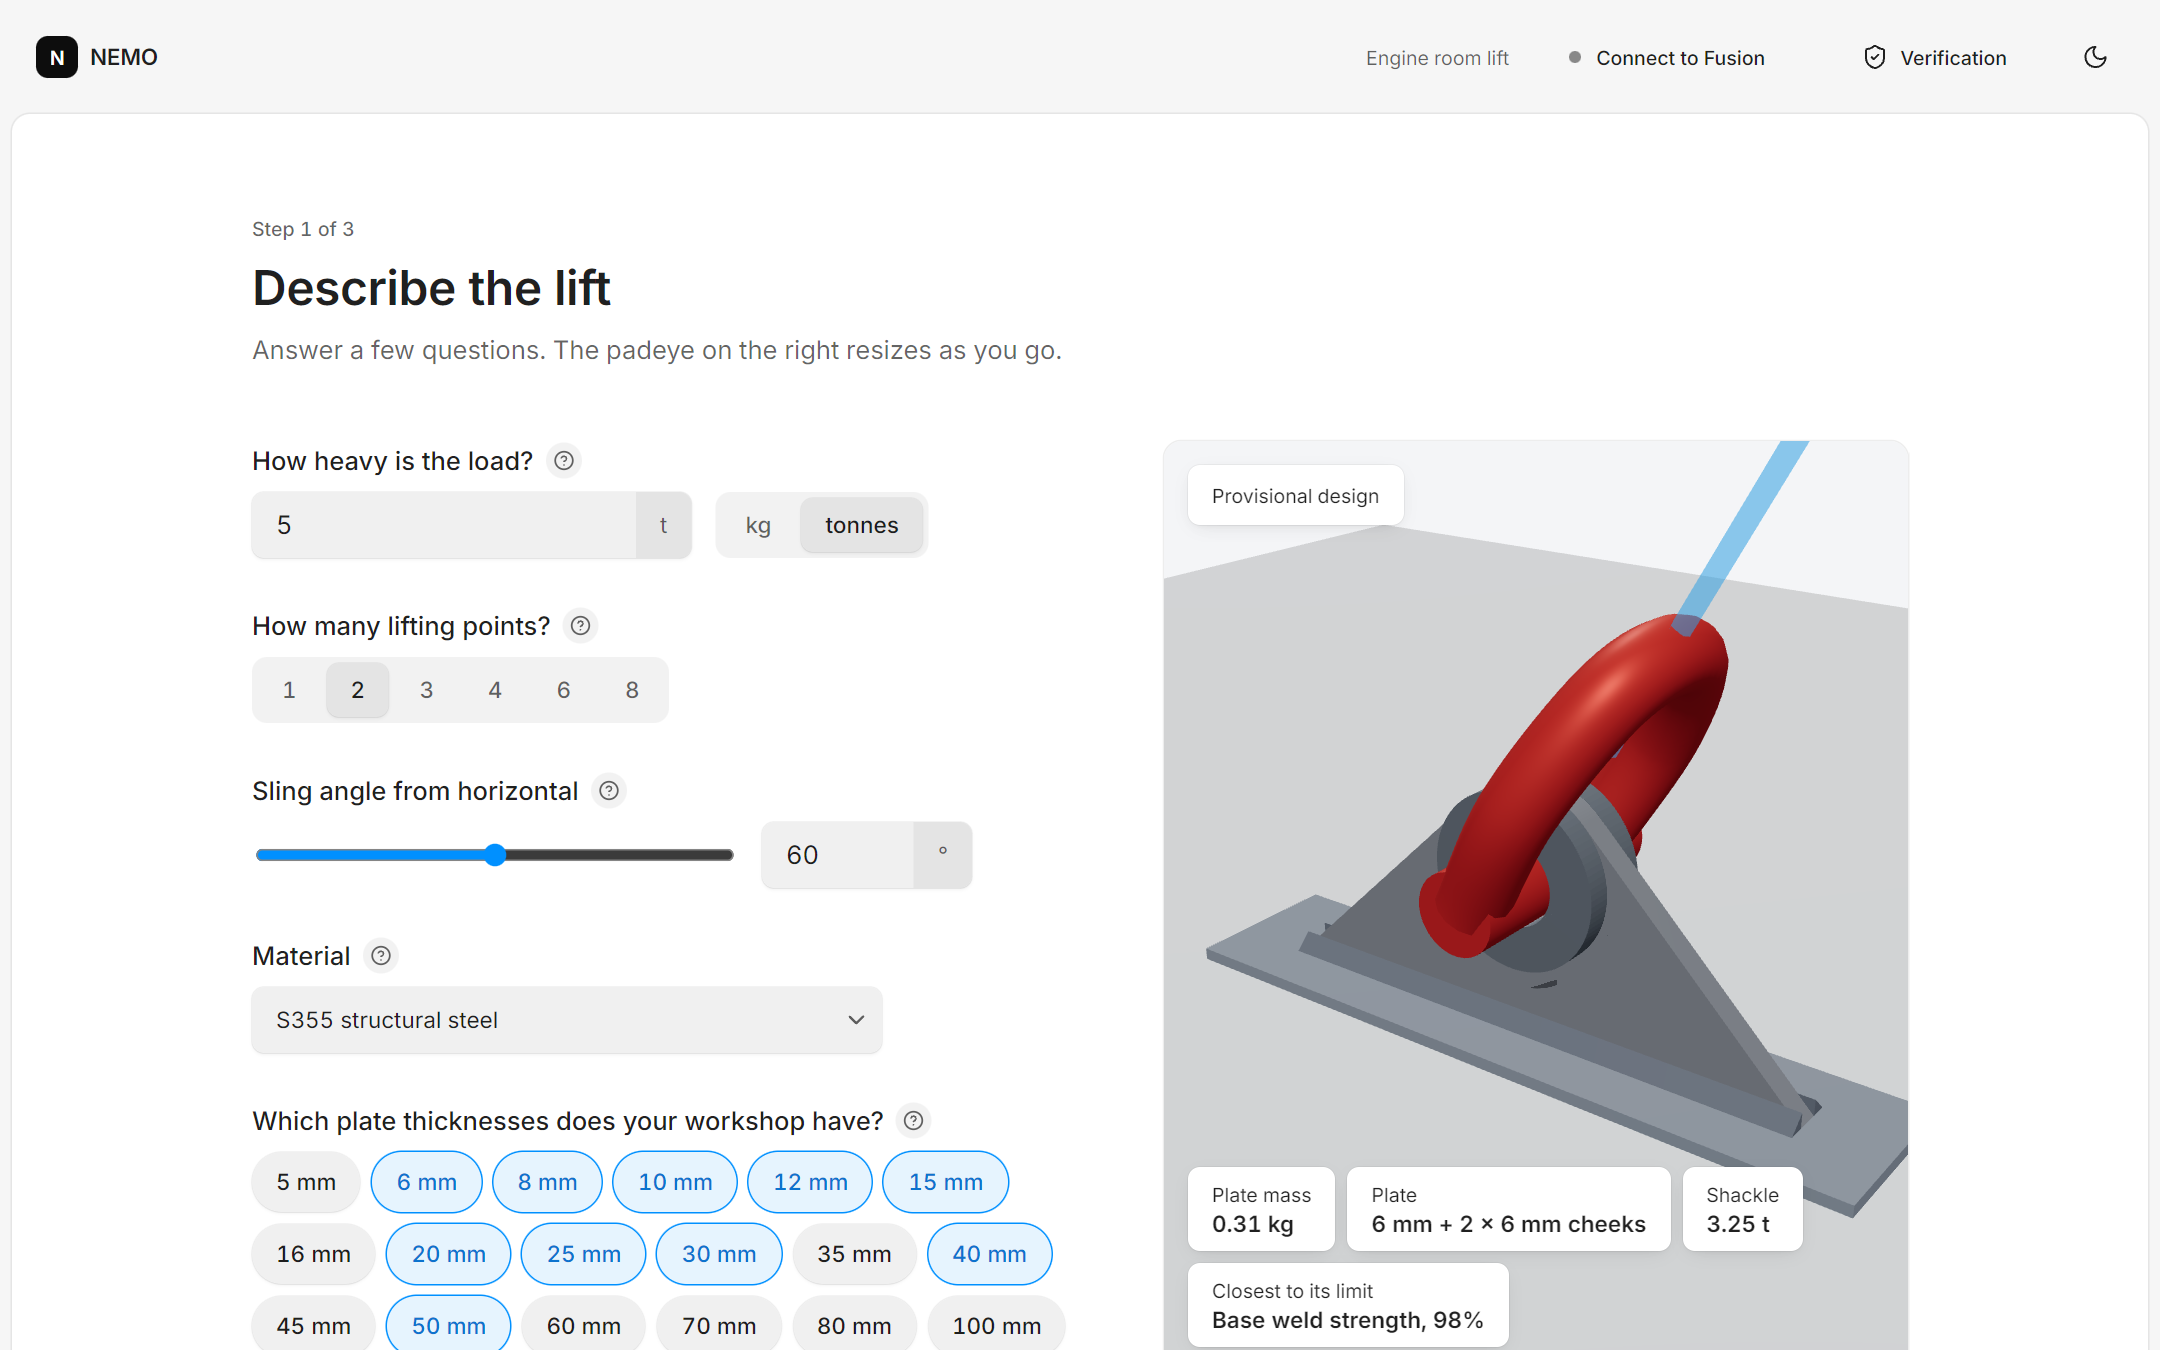
\includegraphics[width=\textwidth]{images/app-padeye-describe.png}
\caption{Job description form for a lifting padeye with the live 3D preview}
\label{fig:app-describe}
\end{figure}

\begin{figure}[H]
\centering
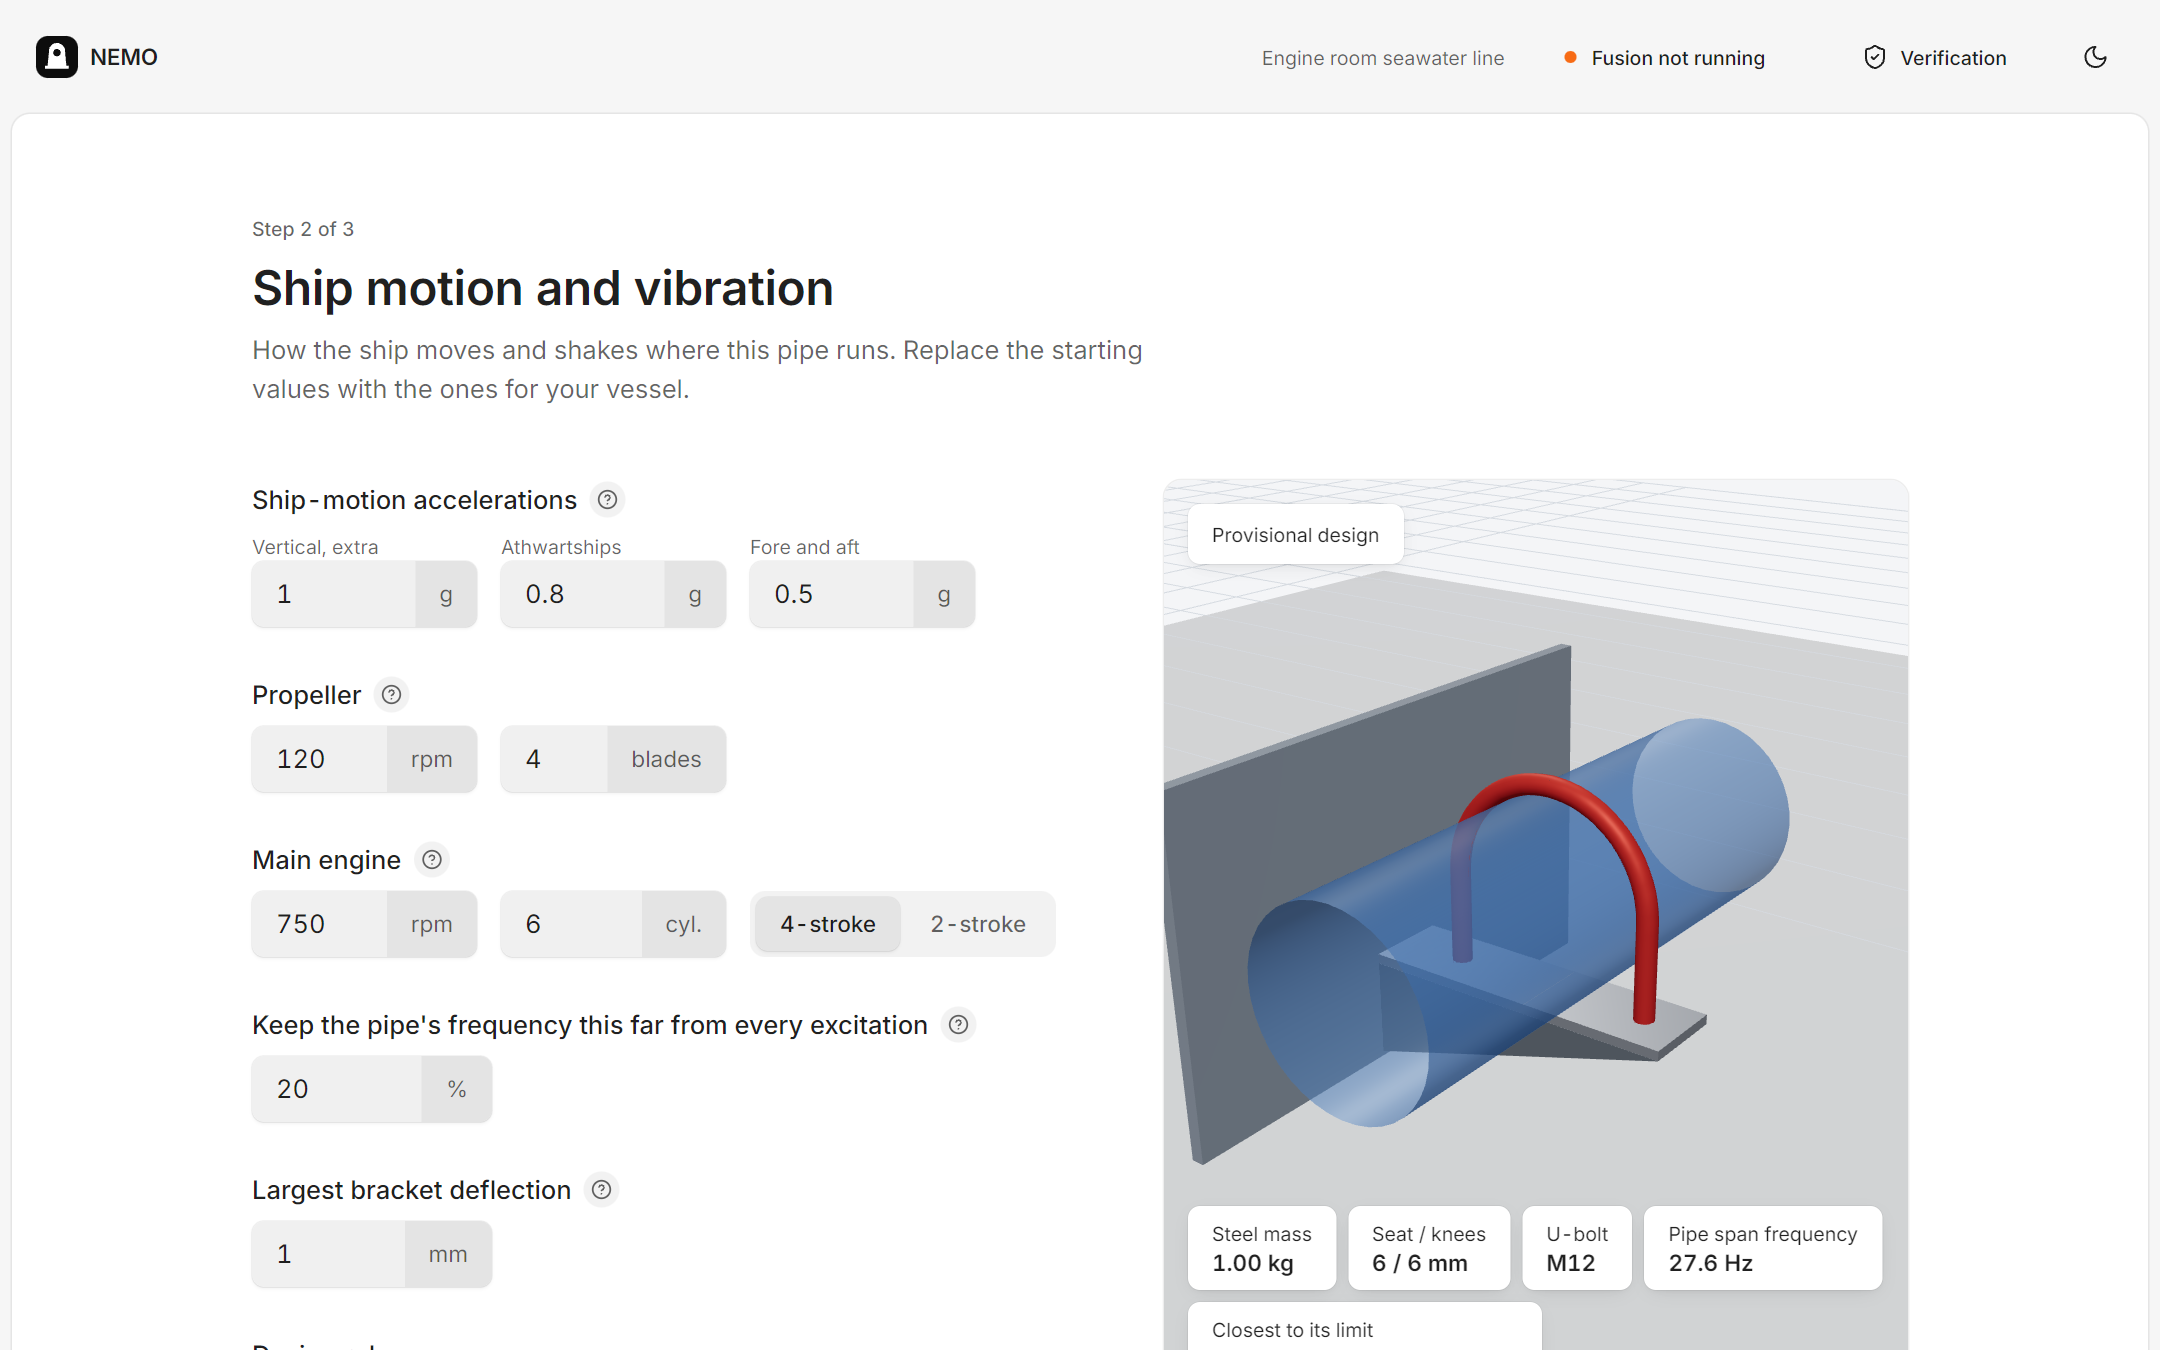
\includegraphics[width=\textwidth]{images/app-bracket-motion.png}
\caption{Ship motion and machinery vibration form for a pipe support bracket}
\label{fig:app-bracket-motion}
\end{figure}

\begin{figure}[H]
\centering
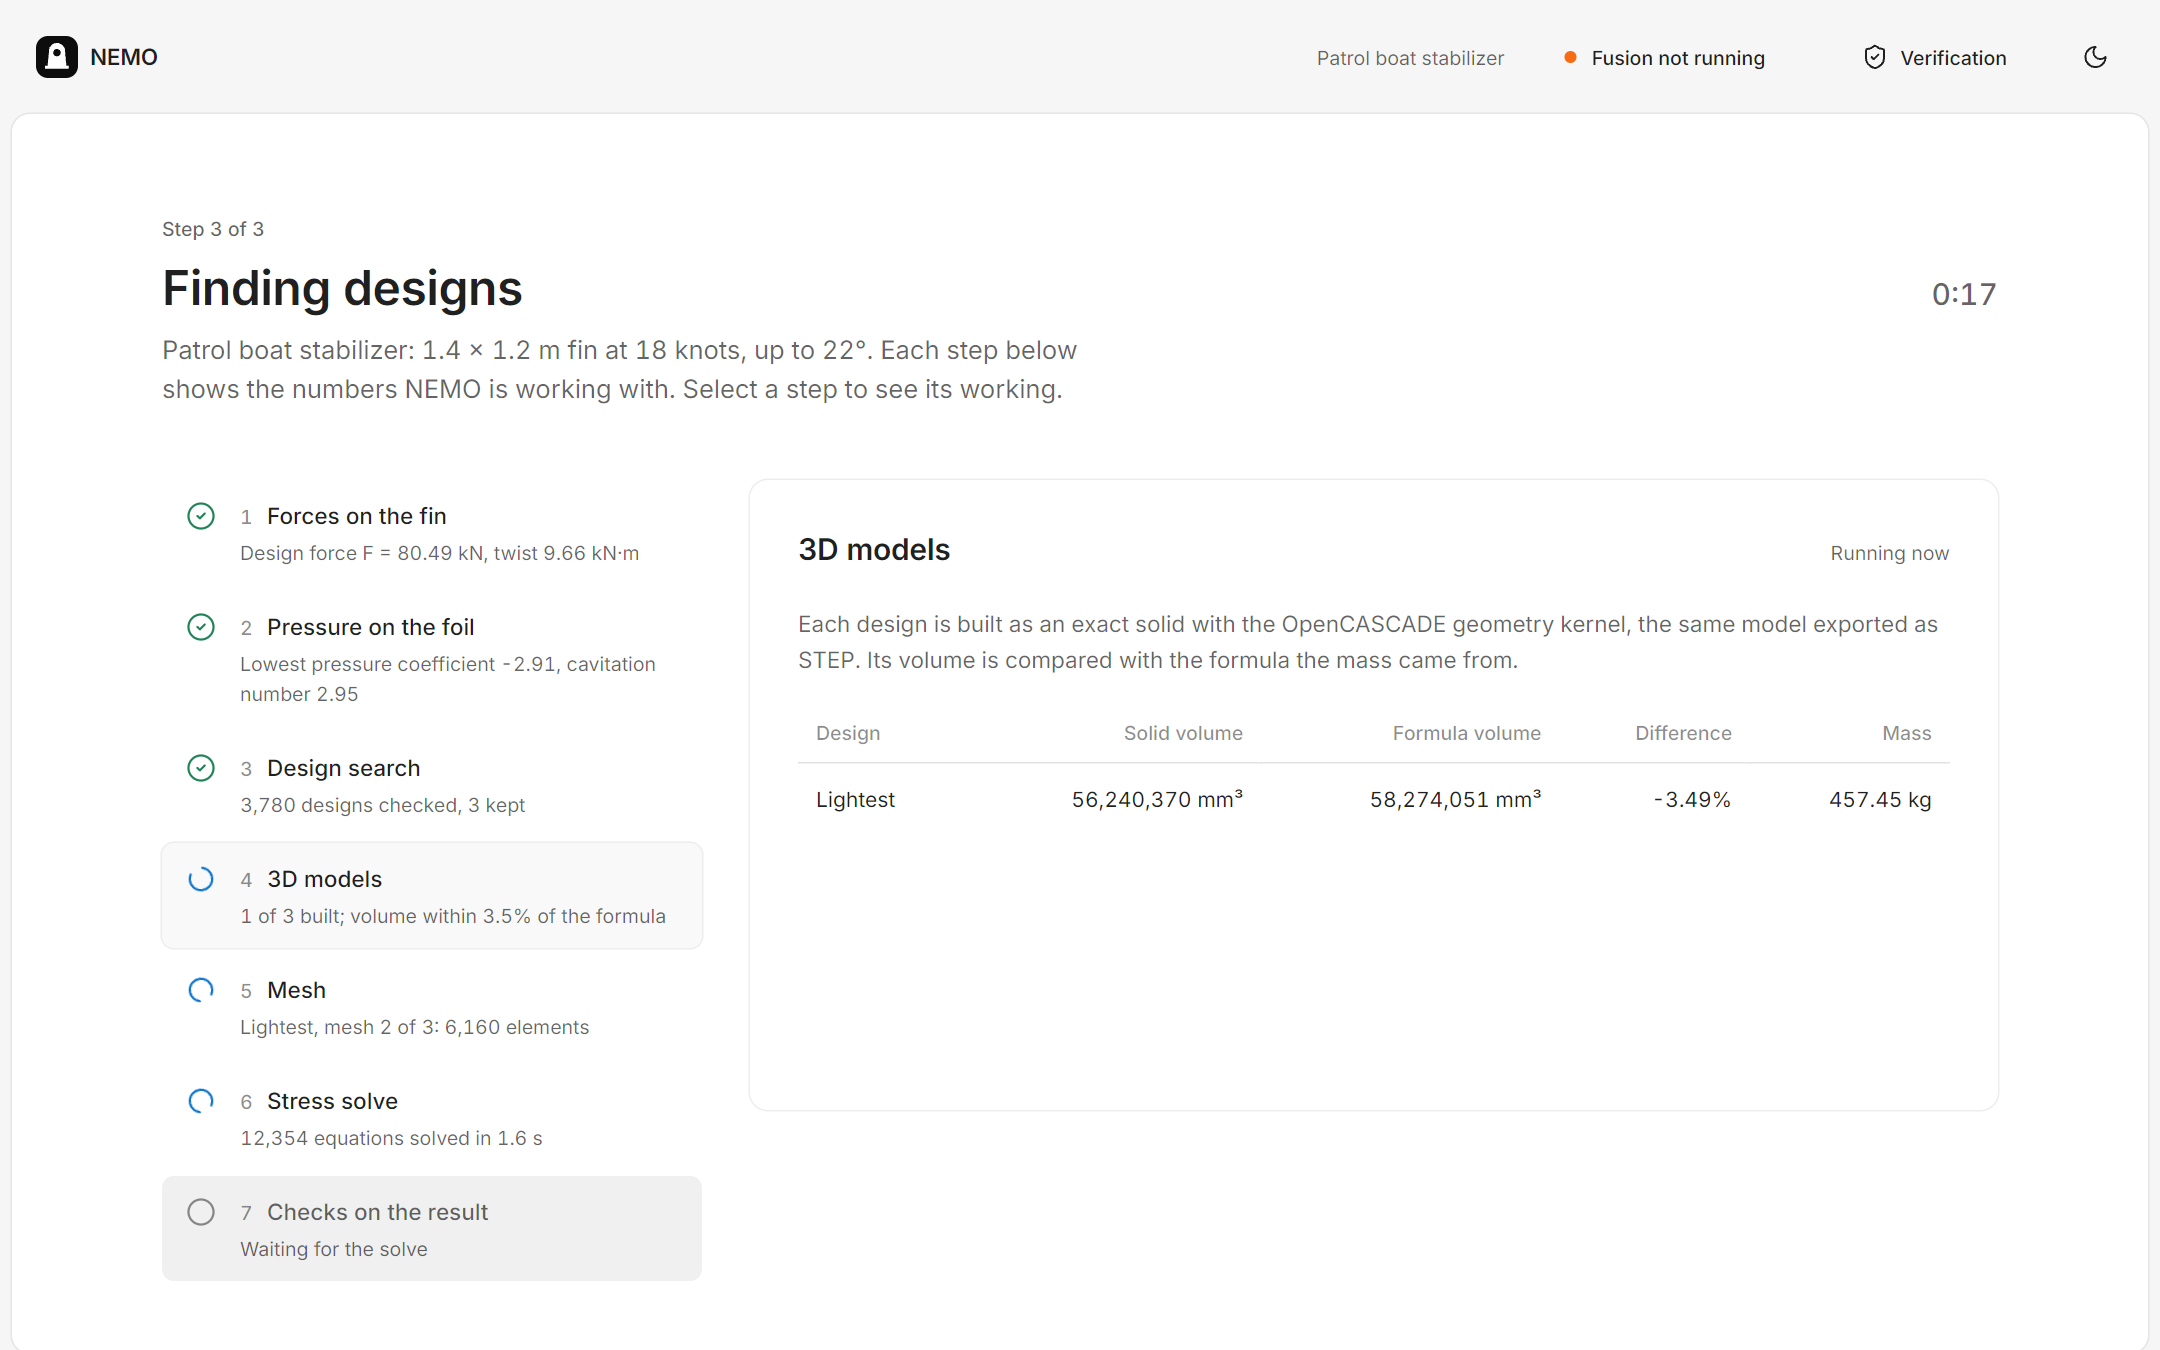
\includegraphics[width=\textwidth]{images/app-running.png}
\caption{Live run screen during the fin case study, with the 3D model step
selected}
\label{fig:app-running}
\end{figure}

\section{Fusion connector}
\label{sec:fusion-connector}

The Fusion connector is an optional add-in for Autodesk Fusion that works with
padeyes. Rather than writing persistent request files that can rebuild stale
geometry on startup, it polls the local \NEMO{} server over HTTP every 1.5~s. A
job that is not picked up within 45~s, or not finished within 180~s, expires,
and each job is handed out only once, which answers requirement R8.

When the user sends a design to Fusion, the add-in builds a parametric model.
The dimensions are user parameters named \code{nemo\_t}, \code{nemo\_R},
\code{nemo\_Dh}, \code{nemo\_L}, \code{nemo\_h}, \code{nemo\_tc} and
\code{nemo\_Rc}, bound to the sketch dimensions and extrusions, so the design
can be edited in Fusion's parameter table. The add-in assigns the material,
names the hole and base faces, and reports Fusion's volume back to \NEMO{} for
comparison with its own. Fusion's material library holds American AISI and
ASTM grades but none of the EN or IACS grades \NEMO{} uses, and its generic
\emph{Steel} has a yield strength of 207~MPa. The add-in (version 1.1.1)
therefore copies \emph{Steel} into the design, names the copy after the
\NEMO{} grade, converts and assigns its modulus, Poisson's ratio, density,
yield and ultimate strength (guarding against Fusion's negative unit-conversion
error sentinel and empty property units), and reads every value back. \NEMO{}
records whether they match, and the cross-check sheet gives manual steps if
they do not. A \emph{Check in NEMO} command sends edited parameters back, and
\NEMO{} re-runs every check and displays the results inside Fusion.

Fusion's API cannot create or solve a Simulation study \cite{autodeskAddins},
so a Fusion stress cross-check is set up by hand using a sheet that \NEMO{}
generates with the loads, supports and material. The engineer enters Fusion's
total reaction and peak stress, and \NEMO{} counts the two analyses as agreeing
when the reaction is within 2\% of the applied load and the peak stress near
the hole is within 15\% of \NEMO{}'s. A reaction less than half or more than
1.5 times the applied load is refused and not recorded: a fixed support always
carries the whole load, so such a value can only have been read from the wrong
result. The sheet lists the three-dimensional resultant and all three load
components, specifies both a global mesh size and a local hole mesh size, and
warns the engineer to probe on the inner pin-hole surface rather than reading
the legend maximum at the fixed base corners or at an unmodeled 90$^\circ$
cheek-plate step. The record is added to section~7 of the PDF. The server side
of the connector, including the job queue, job expiry, unit-conversion guards
and the material record, is covered by the automated tests.
Section~\ref{sec:fusion-session} reports the initial Fusion cross-check trial.

The connector builds padeyes only. For brackets and fins, section~8 of their
calculation packages lists the same values for a cross-check by hand from the
STEP file, including the material values, the load face to split off and the
fin's twisting moment. For the fin it uses \code{fin-stock.step}, because
\NEMO{}'s stress check models the stock alone.

\section{Case studies}
\label{sec:case-studies}

One case per part was chosen to be typical of work in a small yard or an
engine room refit. Table~\ref{tab:cases} gives the inputs. All three were run
with the default plate stock of the material and the default settings
otherwise. For the advanced settings this means a padeye lined up with its
sling ($\beta = 0^\circ$), the bracket's flexibility included, the fin's
astern condition included at the rule's least astern speed of 9~knots, and the
fin's bearing check off. Section~\ref{sec:advanced-results} then uses the
advanced settings on the same cases. The results are in
Chapter~\ref{chap:results}.

\begin{table}[H]
\centering
\caption{Case-study inputs}
\label{tab:cases}
\small
\begin{tabularx}{\textwidth}{>{\raggedright\arraybackslash}p{0.17\textwidth}>{\raggedright\arraybackslash}X}
\toprule
\textbf{Case} & \textbf{Inputs}\\
\midrule
Engine room lift (padeye) & 5~t lifted on two padeyes, sling angle 60$^\circ$, dynamic factor 1.0, sideways allowance 5\%, S355 plate from 6~mm to 50~mm, cheek plates allowed, BTH-1 design category~B, service class~0, E70XX electrodes\\
Engine room seawater line (bracket) & NPS~4 STD carbon steel pipe full of sea water, no insulation, 3~m spacing, continuity factor 1.25, fore-and-aft pipe, accelerations 1.0~g vertical, 0.8~g athwartships and 0.5~g fore-and-aft, friction 0.3, 50~mm gap to the bulkhead, Grade~A plate from 6~mm to 20~mm, class 4.6 U-bolt, propeller 120~rpm with 4 blades, six-cylinder four-stroke engine at 750~rpm, 20\% frequency margin, 1~mm deflection limit\\
Patrol boat stabilizer (fin) & 1.4~m span, 1.2~m chord, NACA~0020, 18~knots, largest angle 22$^\circ$, stock at 35\% chord, spars at 15\% and 65\% chord, fin 3~m below the surface, draught 5~m, 200~mm root-to-bearing gap, AH36 plate from 8~mm to 25~mm, 42CrMo4 stock, 10~mm tip deflection limit\\
\bottomrule
\end{tabularx}
\end{table}

Parameter sweeps were run on the same cases to see how the designs respond.
The padeye was sized for loads of 1~t to 40~t at sling angles of 45$^\circ$,
60$^\circ$ and 90$^\circ$. The bracket was run for pipe sizes NPS~2 to NPS~12,
and its pipe span for spacings of 1.5~m to 6~m. The fin was sized for speeds
of 10 to 24~knots. The data and scripts that produce every figure and number
in Chapter~\ref{chap:results} are kept with this report, in \code{data/} and
\code{tools/}, so the results can be regenerated.
